%%%%%%%%%%%%%%%%%%%%%%%%%%%%%%%%%%%%%%%%
% The Legrand Orange Book
% LaTeX Template
% Version 2.1.1 (14/2/16)
%
% This template has been downloaded from:
% http://www.LaTeXTemplates.com
%
% Original author:
% Mathias Legrand (legrand.mathias@gmail.com) with modifications by:
% Vel (vel@latextemplates.com)
%
% It has been modified by Anders Bergman (anders.bergman@physics.uu.se)
% by adding additional macros, changed color scheme and added environments.
%
% The file has been updated by Manuel Pereiro (manuel.pereiro@physics.uu.se) 
% to comply with the $\mu$ASD manual and new macros.
% License:
% CC BY-NC-SA 3.0 (http://creativecommons.org/licenses/by-nc-sa/3.0/)
%
% Compiling this template:
% This template does not use biber for its bibliography but makeindex for its index.
% When you first open the template, compile it from the command line with the 
% commands below to make sure your LaTeX distribution is configured correctly:
%
% 1) pdflatex main
% 2) makeindex main.idx -s StyleInd.ist
% 3) #biber main
% 4) pdflatex main x 2
%
% After this, when you wish to update the bibliography/index use the appropriate
% command above and make sure to compile with pdflatex several times 
% afterwards to propagate your changes to the document.
%
% This template also uses a number of packages which may need to be
% updated to the newest versions for the template to compile. It is strongly
% recommended you update your LaTeX distribution if you have any
% compilation errors.
%
% Important note:
% Chapter heading images should have a 2:1 width:height ratio,
% e.g. 920px width and 460px height.
%
%%%%%%%%%%%%%%%%%%%%%%%%%%%%%%%%%%%%%%%%%

%----------------------------------------------------------------------------------------
%	PACKAGES AND OTHER DOCUMENT CONFIGURATIONS
%----------------------------------------------------------------------------------------

\documentclass[11pt,fleqn,a4]{book} % Default font size and left-justified equations
\usepackage[utf8]{inputenc}
\usepackage{fancyvrb}
\usepackage{amsmath}
\usepackage{mathrsfs}
\usepackage{ulem}
\usepackage{calc}  
\usepackage{listings}% http://ctan.org/pkg/listings
\usepackage{underscore}
\usepackage[caption=false]{subfig}
\usepackage{underscore}

%. Graphics and style
\usepackage{graphicx}
\usepackage{xcolor}
\usepackage{transparent}
%\usepackage[adobe-utopia]{mathdesign}
\usepackage{color}
\usepackage{epstopdf} %converting to PDF
\usepackage{placeins}
\usepackage{courier}
\usepackage{caption}
\usepackage{dirtree}
\usepackage{multicol}
\graphicspath{Pictures/}

%. listing style

\definecolor{codegreen}{rgb}{0,0.6,0}
\definecolor{codegray}{rgb}{0.5,0.5,0.5}
\definecolor{codepurple}{rgb}{0.58,0,0.82}
\colorlet{Mycolor1}{black!5}

\lstdefinestyle{mystyle}{
    backgroundcolor=\color{Mycolor1},   
    commentstyle=\color{codegreen},
    keywordstyle=\color{magenta},
    numberstyle=\tiny\color{codegray},
    stringstyle=\color{codepurple},
    basicstyle=\ttfamily\footnotesize,
    breakatwhitespace=false,         
    breaklines=true,                 
    captionpos=b,                    
    keepspaces=true,                 
    numbers=left,                    
    numbersep=5pt,                  
    showspaces=false,                
    showstringspaces=false,
    showtabs=false,                  
    tabsize=2
}

\lstset{style=mystyle}
%Macros that are useful when editing the manual. (AB)
 
%Prints keywords bold and add them to index and as label
\newcommand{\litem}[1]{\item[\bfseries#1\index{#1@\texttt{#1}}\label{#1}]}
%References keywords in text
\newcommand{\keyword}[1]{\hyperref[#1]{\texttt{#1}}\index{#1@\texttt{#1}}\label{#1}}
\newcommand{\keywordl}[1]{\texttt{#1}}
%References filenames in text
\newcommand{\rfilename}[1]{\hyperref[#1]{\texttt{#1}}}
%Adds file names to index and as label
\newcommand{\vindex}[1]{\index{#1@\texttt{#1}}\label{#1}}
% New definition of different variables
\newcommand{\name}[1]{#1}
\newcommand{\syntline}[1]{\noindent\\[3pt]\mbox{\texttt{#1}}\\[3pt]}

%----------------------------------------------------------------------------------------

%%%%%%%%%%%%%%%%%%%%%%%%%%%%%%%%%%%%%%%%%
% The Legrand Orange Book
% Structural Definitions File
% Version 2.0 (9/2/15)
%
% Original author:
% Mathias Legrand (legrand.mathias@gmail.com) with modifications by:
% Vel (vel@latextemplates.com)
% 
% This file has been downloaded from:
% http://www.LaTeXTemplates.com
%
% License:
% CC BY-NC-SA 3.0 (http://creativecommons.org/licenses/by-nc-sa/3.0/)
%
%%%%%%%%%%%%%%%%%%%%%%%%%%%%%%%%%%%%%%%%%

%----------------------------------------------------------------------------------------
%	VARIOUS REQUIRED PACKAGES AND CONFIGURATIONS
%----------------------------------------------------------------------------------------

\usepackage[top=3cm,bottom=3cm,left=3cm,right=3cm,headsep=10pt,a4paper]{geometry} % Page margins

\usepackage{graphicx} % Required for including pictures
\graphicspath{{Pictures/}} % Specifies the directory where pictures are stored

\usepackage{lipsum} % Inserts dummy text

\usepackage{tikz} % Required for drawing custom shapes

\usepackage[english]{babel} % English language/hyphenation

\usepackage{booktabs} % Required for nicer horizontal rules in tables

\usepackage{xcolor} % Required for specifying colors by name
%\definecolor{ocre}{RGB}{243,102,25} % Define the orange color used for highlighting throughout the book
\definecolor{ocre}{RGB}{160,25,25} % Define the orange color used for highlighting throughout the book
\definecolor{grey}{RGB}{50,50,50} % Define the grey color

%----------------------------------------------------------------------------------------
%	FONTS
%----------------------------------------------------------------------------------------

\usepackage{avant} % Use the Avantgarde font for headings
%\usepackage{times} % Use the Times font for headings
\usepackage{mathptmx} % Use the Adobe Times Roman as the default text font together with math symbols from the Sym­bol, Chancery and Com­puter Modern fonts

\usepackage{microtype} % Slightly tweak font spacing for aesthetics
\usepackage[utf8]{inputenc} % Required for including letters with accents
\usepackage[T1]{fontenc} % Use 8-bit encoding that has 256 glyphs

%----------------------------------------------------------------------------------------
%	BIBLIOGRAPHY AND INDEX
%----------------------------------------------------------------------------------------

%\usepackage[style=alphabetic,citestyle=numeric,sorting=nyt,sortcites=true,autopunct=true,babel=hyphen,hyperref=true,abbreviate=false,backref=true,backend=biber]{biblatex}
%\addbibresource{bibliography.bib} % BibTeX bibliography file
%\defbibheading{bibempty}{}
\usepackage{calc} % For simpler calculation - used for spacing the index letter headings correctly
\usepackage{hyperref}
\usepackage{cleveref}
\usepackage{cite}
\usepackage{makeidx} % Required to make an index
\usepackage{enumitem} % Customize lists

\setlist{nolistsep} % Reduce spacing between bullet points and numbered lists

\makeindex % Tells LaTeX to create the files required for indexing

%----------------------------------------------------------------------------------------
%	MAIN TABLE OF CONTENTS
%----------------------------------------------------------------------------------------

\usepackage{titletoc} % Required for manipulating the table of contents

\contentsmargin{0cm} % Removes the default margin

% Part text styling
\titlecontents{part}[0cm]
{\addvspace{20pt}\centering\large\bfseries}
{}
{}
{}

% Chapter text styling
\titlecontents{chapter}[1.25cm] % Indentation
{\addvspace{12pt}\large\sffamily\bfseries} % Spacing and font options for chapters
{\color{ocre!60}\contentslabel[\Large\thecontentslabel]{1.25cm}\color{ocre}} % Chapter number
{\color{ocre}}  
{\color{ocre!60}\normalsize\;\titlerule*[.5pc]{.}\;\thecontentspage} % Page number

% Section text styling
\titlecontents{section}[1.25cm] % Indentation
{\addvspace{3pt}\sffamily\bfseries} % Spacing and font options for sections
{\contentslabel[\thecontentslabel]{1.25cm}} % Section number
{}
{\hfill\color{black}\thecontentspage} % Page number
[]

% Subsection text styling
\titlecontents{subsection}[1.25cm] % Indentation
{\addvspace{1pt}\sffamily\small} % Spacing and font options for subsections
{\contentslabel[\thecontentslabel]{1.25cm}} % Subsection number
{}
{\ \titlerule*[.5pc]{.}\;\thecontentspage} % Page number
[]

% List of figures
\titlecontents{figure}[0em]
{\addvspace{-5pt}\sffamily}
{\thecontentslabel\hspace*{1em}}
{}
{\ \titlerule*[.5pc]{.}\;\thecontentspage}
[]

% List of tables
\titlecontents{table}[0em]
{\addvspace{-5pt}\sffamily}
{\thecontentslabel\hspace*{1em}}
{}
{\ \titlerule*[.5pc]{.}\;\thecontentspage}
[]

%----------------------------------------------------------------------------------------
%	MINI TABLE OF CONTENTS IN PART HEADS
%----------------------------------------------------------------------------------------

% Chapter text styling
\titlecontents{lchapter}[0em] % Indenting
{\addvspace{15pt}\large\sffamily\bfseries} % Spacing and font options for chapters
{\color{ocre}\contentslabel[\Large\thecontentslabel]{1.25cm}\color{ocre}} % Chapter number
{}  
{\color{ocre}\normalsize\sffamily\bfseries\;\titlerule*[.5pc]{.}\;\thecontentspage} % Page number

% Section text styling
\titlecontents{lsection}[0em] % Indenting
{\sffamily\small} % Spacing and font options for sections
{\contentslabel[\thecontentslabel]{1.25cm}} % Section number
{}
{}

% Subsection text styling
\titlecontents{lsubsection}[.5em] % Indentation
{\normalfont\footnotesize\sffamily} % Font settings
{}
{}
{}

%----------------------------------------------------------------------------------------
%	PAGE HEADERS
%----------------------------------------------------------------------------------------

\usepackage{fancyhdr} % Required for header and footer configuration

\pagestyle{fancy}
\renewcommand{\chaptermark}[1]{\markboth{\sffamily\normalsize\bfseries\chaptername\ \thechapter.\ #1}{}} % Chapter text font settings
\renewcommand{\sectionmark}[1]{\markright{\sffamily\normalsize\thesection\hspace{5pt}#1}{}} % Section text font settings
\fancyhf{} \fancyhead[LE,RO]{\sffamily\normalsize\thepage} % Font setting for the page number in the header
\fancyhead[LO]{\rightmark} % Print the nearest section name on the left side of odd pages
\fancyhead[RE]{\leftmark} % Print the current chapter name on the right side of even pages
\renewcommand{\headrulewidth}{0.5pt} % Width of the rule under the header
\addtolength{\headheight}{2.5pt} % Increase the spacing around the header slightly
\renewcommand{\footrulewidth}{0pt} % Removes the rule in the footer
\fancypagestyle{plain}{\fancyhead{}\renewcommand{\headrulewidth}{0pt}} % Style for when a plain pagestyle is specified

% Removes the header from odd empty pages at the end of chapters
\makeatletter
\renewcommand{\cleardoublepage}{
\clearpage\ifodd\c@page\else
\hbox{}
\vspace*{\fill}
\thispagestyle{empty}
\newpage
\fi}

%----------------------------------------------------------------------------------------
%	THEOREM STYLES
%----------------------------------------------------------------------------------------

\usepackage{amsmath,amsfonts,amssymb,amsthm} % For math equations, theorems, symbols, etc

\newcommand{\intoo}[2]{\mathopen{]}#1\,;#2\mathclose{[}}
\newcommand{\ud}{\mathop{\mathrm{{}d}}\mathopen{}}
\newcommand{\intff}[2]{\mathopen{[}#1\,;#2\mathclose{]}}
\newtheorem{notation}{Notation}[chapter]

% Boxed/framed environments
\newtheoremstyle{ocrenumbox}% % Theorem style name
{0pt}% Space above
{0pt}% Space below
{\normalfont}% % Body font
{}% Indent amount
{\small\bf\sffamily\color{ocre}}% % Theorem head font
{\;}% Punctuation after theorem head
{0.25em}% Space after theorem head
{\small\sffamily\color{ocre}\thmname{#1}\nobreakspace\thmnumber{\@ifnotempty{#1}{}\@upn{#2}}% Theorem text (e.g. Theorem 2.1)
\thmnote{\nobreakspace\the\thm@notefont\sffamily\bfseries\color{black}---\nobreakspace#3.}} % Optional theorem note
\renewcommand{\qedsymbol}{$\blacksquare$}% Optional qed square

\newtheoremstyle{blacknumex}% Theorem style name
{5pt}% Space above
{5pt}% Space below
{\normalfont}% Body font
{} % Indent amount
{\small\bf\sffamily}% Theorem head font
{\;}% Punctuation after theorem head
{0.25em}% Space after theorem head
{\small\sffamily{\tiny\ensuremath{\blacksquare}}\nobreakspace\thmname{#1}\nobreakspace\thmnumber{\@ifnotempty{#1}{}\@upn{#2}}% Theorem text (e.g. Theorem 2.1)
\thmnote{\nobreakspace\the\thm@notefont\sffamily\bfseries---\nobreakspace#3.}}% Optional theorem note


\newtheoremstyle{blacknumbox} % Theorem style name
{0pt}% Space above
{0pt}% Space below
{\normalfont}% Body font
{}% Indent amount
{\small\bf\sffamily}% Theorem head font
{\;}% Punctuation after theorem head
{0.25em}% Space after theorem head
{\small\sffamily\thmname{#1}\nobreakspace\thmnumber{\@ifnotempty{#1}{}\@upn{#2}}% Theorem text (e.g. Theorem 2.1)
\thmnote{\nobreakspace\the\thm@notefont\sffamily\bfseries---\nobreakspace#3.}}% Optional theorem note

\newtheoremstyle{blacknonumbox} % Theorem style name
{0pt}% Space above
{0pt}% Space below
{\normalfont}% Body font
{}% Indent amount
{\small\bf\sffamily}% Theorem head font
{\;}% Punctuation after theorem head
{0.25em}% Space after theorem head
{\small\sffamily\thmname{}\nobreakspace{\@ifnotempty{}{}\@upn{}}% Theorem text (e.g. Theorem 2.1)
\thmnote{\nobreakspace#3}}% Optional theorem note


% Non-boxed/non-framed environments
\newtheoremstyle{ocrenum}% % Theorem style name
{5pt}% Space above
{5pt}% Space below
{\normalfont}% % Body font
{}% Indent amount
{\small\bf\sffamily\color{ocre}}% % Theorem head font
{\;}% Punctuation after theorem head
{0.25em}% Space after theorem head
{\small\sffamily\color{ocre}\thmname{#1}\nobreakspace\thmnumber{\@ifnotempty{#1}{}\@upn{#2}}% Theorem text (e.g. Theorem 2.1)
\thmnote{\nobreakspace\the\thm@notefont\sffamily\bfseries\color{black}---\nobreakspace#3.}} % Optional theorem note
\renewcommand{\qedsymbol}{$\blacksquare$}% Optional qed square
\makeatother

% Defines the theorem text style for each type of theorem to one of the three styles above

\newcounter{dummy} 
\numberwithin{dummy}{section}
\theoremstyle{ocrenumbox}
\newtheorem{theoremeT}[dummy]{Theorem}
%\newtheorem{equationT}{Equation}
\newtheorem{equationT}{Equation}
\newtheorem{equationC}[dummy]{Equation}
\newtheorem{alignT}[dummy]{Equation}
\newtheorem{problem}{Problem}[chapter]
\newtheorem{exerciseT}{Exercise}[chapter]
\theoremstyle{blacknumex}
\newtheorem{exampleT}{Example}[chapter]
\theoremstyle{blacknumbox}
\newtheorem{vocabulary}{Vocabulary}[chapter]
\newtheorem{definitionT}{Definition}[section]
\newtheorem{corollaryT}[dummy]{Corollary}
\theoremstyle{ocrenum}
\newtheorem{proposition}[dummy]{Proposition}
\theoremstyle{blacknonumbox}
\newtheorem{declarationT}{}

%----------------------------------------------------------------------------------------
%	DEFINITION OF COLORED BOXES
%----------------------------------------------------------------------------------------

\RequirePackage[framemethod=default]{mdframed} % Required for creating the theorem, definition, exercise and corollary boxes

% Theorem box
\newmdenv[skipabove=7pt,
skipbelow=7pt,
backgroundcolor=black!5,
linecolor=ocre,
innerleftmargin=5pt,
innerrightmargin=5pt,
innertopmargin=5pt,
leftmargin=0cm,
rightmargin=0cm,
nobreak=true,
innerbottommargin=5pt]{tBox}

% Gray theorem box
\newmdenv[skipabove=7pt,
skipbelow=7pt,
backgroundcolor=black!5,
linecolor=black!90,
innerleftmargin=5pt,
innerrightmargin=5pt,
innertopmargin=5pt,
leftmargin=0cm,
rightmargin=0cm,
nobreak=true,
innerbottommargin=5pt]{gBox}


% Exercise box	  
\newmdenv[skipabove=7pt,
skipbelow=7pt,
rightline=false,
leftline=true,
topline=false,
bottomline=false,
backgroundcolor=ocre!10,
linecolor=ocre,
innerleftmargin=5pt,
innerrightmargin=5pt,
innertopmargin=5pt,
innerbottommargin=5pt,
leftmargin=0cm,
rightmargin=0cm,
linewidth=4pt]{eBox}	

% Definition box
\newmdenv[skipabove=7pt,
skipbelow=7pt,
rightline=false,
leftline=true,
topline=false,
bottomline=false,
linecolor=ocre,
innerleftmargin=5pt,
innerrightmargin=5pt,
innertopmargin=0pt,
leftmargin=0cm,
rightmargin=0cm,
linewidth=4pt,
innerbottommargin=0pt]{dBox}	

% Corollary box
\newmdenv[skipabove=7pt,
skipbelow=7pt,
rightline=false,
leftline=true,
topline=false,
bottomline=false,
linecolor=gray,
backgroundcolor=black!5,
innerleftmargin=5pt,
innerrightmargin=5pt,
innertopmargin=5pt,
leftmargin=0cm,
rightmargin=0cm,
linewidth=4pt,
innerbottommargin=5pt]{cBox}

% Text box
\newmdenv[skipabove=7pt,
skipbelow=7pt,
rightline=false,
leftline=false,
topline=false,
bottomline=false,
linecolor=gray,
backgroundcolor=black!5,
innerleftmargin=5pt,
innerrightmargin=5pt,
innertopmargin=5pt,
leftmargin=0cm,
rightmargin=0cm,
linewidth=4pt,
innerbottommargin=5pt]{fBox}

% Creates an environment for each type of theorem and assigns it a theorem text style from the "Theorem Styles" section above and a colored box from above
\newenvironment{theorem}{\begin{tBox}\begin{theoremeT}}{\end{theoremeT}\end{tBox}}
\newenvironment{equationD}{\begin{tBox} \begin{equationC} }{ \end{equationC}\end{tBox}}
\newenvironment{equationB}{\begin{tBox} \begin{equationT} }{ \end{equationT}\end{tBox}}
%\newenvironment{equationB}{\begin{tBox}\begin{equationT}\begin{center}\begin{equation}}{\end{equation}\end{center}\end{equationT}\end{tBox}}
\newenvironment{alignB}{\begin{tBox}\begin{alignT}\begin{center}\begin{equation}}{\end{equation}\end{center}\end{alignT}\end{tBox}}
\newenvironment{exercise}{\begin{eBox}\begin{exerciseT}}{\hfill{\color{ocre}\tiny\ensuremath{\blacksquare}}\end{exerciseT}\end{eBox}}				  
\newenvironment{definition}{\begin{dBox}\begin{definitionT}}{\end{definitionT}\end{dBox}}	
\newenvironment{declaration}{\begin{dBox}\begin{declarationT}}{\end{declarationT}\end{dBox}}	
\newenvironment{example}{\begin{exampleT}}{\hfill{\tiny\ensuremath{\blacksquare}}\end{exampleT}}		
\newenvironment{corollary}{\begin{cBox}\begin{corollaryT}}{\end{corollaryT}\end{cBox}}	
\newenvironment{fileinfo}{\begin{cBox}\begin{declarationT}}{\end{declarationT}\end{cBox}}	
%\newenvironment{textinfo}{\begin{tBox}\begin{lstlisting}}{\end{lstlisting}\end{tBox}}	

%----------------------------------------------------------------------------------------
%	REMARK ENVIRONMENT
%----------------------------------------------------------------------------------------

\newenvironment{remark}{\par\vspace{10pt}\small % Vertical white space above the remark and smaller font size
\begin{list}{}{
\leftmargin=35pt % Indentation on the left
\rightmargin=25pt}\item\ignorespaces % Indentation on the right
\makebox[-2.5pt]{\begin{tikzpicture}[overlay]
\node[draw=ocre!60,line width=1pt,circle,fill=ocre!25,font=\sffamily\bfseries,inner sep=2pt,outer sep=0pt] at (-15pt,0pt){\textcolor{ocre}{R}};\end{tikzpicture}} % Orange R in a circle
\advance\baselineskip -1pt}{\end{list}\vskip5pt} % Tighter line spacing and white space after remark

%----------------------------------------------------------------------------------------
%	SECTION NUMBERING IN THE MARGIN
%----------------------------------------------------------------------------------------

\makeatletter
\renewcommand{\@seccntformat}[1]{\llap{\textcolor{ocre}{\csname the#1\endcsname}\hspace{1em}}}                    
\renewcommand{\section}{\@startsection{section}{1}{\z@}
{-4ex \@plus -1ex \@minus -.4ex}
{1ex \@plus.2ex }
{\normalfont\large\sffamily\bfseries}}
\renewcommand{\subsection}{\@startsection {subsection}{2}{\z@}
{-3ex \@plus -0.1ex \@minus -.4ex}
{0.5ex \@plus.2ex }
{\normalfont\sffamily\bfseries}}
\renewcommand{\subsubsection}{\@startsection {subsubsection}{3}{\z@}
{-2ex \@plus -0.1ex \@minus -.2ex}
{.2ex \@plus.2ex }
{\normalfont\small\sffamily\bfseries}}                        
\renewcommand\paragraph{\@startsection{paragraph}{4}{\z@}
{-2ex \@plus-.2ex \@minus .2ex}
{.1ex}
{\normalfont\small\sffamily\bfseries}}

%----------------------------------------------------------------------------------------
%	PART HEADINGS
%----------------------------------------------------------------------------------------

% numbered part in the table of contents
\newcommand{\@mypartnumtocformat}[2]{%
\setlength\fboxsep{0pt}%
\noindent\colorbox{ocre!20}{\strut\parbox[c][.7cm]{\ecart}{\color{ocre!70}\Large\sffamily\bfseries\centering#1}}\hskip\esp\colorbox{ocre!40}{\strut\parbox[c][.7cm]{\linewidth-\ecart-\esp}{\Large\sffamily\centering#2}}}%
%%%%%%%%%%%%%%%%%%%%%%%%%%%%%%%%%%
% unnumbered part in the table of contents
\newcommand{\@myparttocformat}[1]{%
\setlength\fboxsep{0pt}%
\noindent\colorbox{ocre!40}{\strut\parbox[c][.7cm]{\linewidth}{\Large\sffamily\centering#1}}}%
%%%%%%%%%%%%%%%%%%%%%%%%%%%%%%%%%%
\newlength\esp
\setlength\esp{4pt}
\newlength\ecart
\setlength\ecart{1.2cm-\esp}
\newcommand{\thepartimage}{}%
\newcommand{\partimage}[1]{\renewcommand{\thepartimage}{#1}}%
\def\@part[#1]#2{%
\ifnum \c@secnumdepth >-2\relax%
\refstepcounter{part}%
\addcontentsline{toc}{part}{\texorpdfstring{\protect\@mypartnumtocformat{\thepart}{#1}}{\partname~\thepart\ ---\ #1}}
\else%
\addcontentsline{toc}{part}{\texorpdfstring{\protect\@myparttocformat{#1}}{#1}}%
\fi%
\startcontents%
\markboth{}{}%
{\thispagestyle{empty}%
\begin{tikzpicture}[remember picture,overlay]%
\node at (current page.north west){\begin{tikzpicture}[remember picture,overlay]%	
\fill[ocre!20](0cm,0cm) rectangle (\paperwidth,-\paperheight);
\node[anchor=north] at (4cm,-3.25cm){\color{ocre!40}\fontsize{220}{100}\sffamily\bfseries\@Roman\c@part}; 
\node[anchor=south east] at (\paperwidth-1cm,-\paperheight+1cm){\parbox[t][][t]{8.5cm}{
\printcontents{l}{0}{\setcounter{tocdepth}{1}}%
}};
\node[anchor=north east] at (\paperwidth-1.5cm,-3.25cm){\parbox[t][][t]{15cm}{\strut\raggedleft\color{white}\fontsize{30}{30}\sffamily\bfseries#2}};
\end{tikzpicture}};
\end{tikzpicture}}%
\@endpart}
\def\@spart#1{%
\startcontents%
\phantomsection
{\thispagestyle{empty}%
\begin{tikzpicture}[remember picture,overlay]%
\node at (current page.north west){\begin{tikzpicture}[remember picture,overlay]%	
\fill[ocre!20](0cm,0cm) rectangle (\paperwidth,-\paperheight);
\node[anchor=north east] at (\paperwidth-1.5cm,-3.25cm){\parbox[t][][t]{15cm}{\strut\raggedleft\color{white}\fontsize{30}{30}\sffamily\bfseries#1}};
\end{tikzpicture}};
\end{tikzpicture}}
\addcontentsline{toc}{part}{\texorpdfstring{%
\setlength\fboxsep{0pt}%
\noindent\protect\colorbox{ocre!40}{\strut\protect\parbox[c][.7cm]{\linewidth}{\Large\sffamily\protect\centering #1\quad\mbox{}}}}{#1}}%
\@endpart}
\def\@endpart{\vfil\newpage
\if@twoside
\if@openright
\null
\thispagestyle{empty}%
\newpage
\fi
\fi
\if@tempswa
\twocolumn
\fi}

%----------------------------------------------------------------------------------------
%	CHAPTER HEADINGS
%----------------------------------------------------------------------------------------

% A switch to conditionally include a picture, implemented by  Christian Hupfer
\newif\ifusechapterimage
\usechapterimagetrue
\newcommand{\thechapterimage}{}%
\newcommand{\chapterimage}[1]{\ifusechapterimage\renewcommand{\thechapterimage}{#1}\fi}%
\def\@makechapterhead#1{%
{\parindent \z@ \raggedright \normalfont
\ifnum \c@secnumdepth >\m@ne
\if@mainmatter
\begin{tikzpicture}[remember picture,overlay]
\node at (current page.north west)
{\begin{tikzpicture}[remember picture,overlay]
\node[anchor=north west,inner sep=0pt] at (0,0) {\ifusechapterimage\includegraphics[width=\paperwidth]{\thechapterimage}\fi};
\draw[anchor=west] (\Gm@lmargin,-9cm) node [line width=2pt,rounded corners=15pt,draw=ocre,fill=white,fill opacity=0.8,inner sep=15pt]{\strut\makebox[22cm]{}};
\draw[anchor=west] (\Gm@lmargin+.3cm,-9cm) node {\huge\sffamily\bfseries\color{black}\thechapter. #1\strut};
\end{tikzpicture}};
\end{tikzpicture}
\else
\begin{tikzpicture}[remember picture,overlay]
\node at (current page.north west)
{\begin{tikzpicture}[remember picture,overlay]
\node[anchor=north west,inner sep=0pt] at (0,0) {\ifusechapterimage\includegraphics[width=\paperwidth]{\thechapterimage}\fi};
\draw[anchor=west] (\Gm@lmargin,-9cm) node [line width=2pt,rounded corners=15pt,draw=ocre,fill=white,fill opacity=0.8,inner sep=15pt]{\strut\makebox[22cm]{}};
\draw[anchor=west] (\Gm@lmargin+.3cm,-9cm) node {\huge\sffamily\bfseries\color{black}#1\strut};
\end{tikzpicture}};
\end{tikzpicture}
\fi\fi\par\vspace*{270\p@}}}

%-------------------------------------------

\def\@makeschapterhead#1{%
\begin{tikzpicture}[remember picture,overlay]
\node at (current page.north west)
{\begin{tikzpicture}[remember picture,overlay]
\node[anchor=north west,inner sep=0pt] at (0,0) {\ifusechapterimage\includegraphics[width=\paperwidth]{\thechapterimage}\fi};
\draw[anchor=west] (\Gm@lmargin,-9cm) node [line width=2pt,rounded corners=15pt,draw=ocre,fill=white,fill opacity=0.8,inner sep=15pt]{\strut\makebox[22cm]{}};
\draw[anchor=west] (\Gm@lmargin+.3cm,-9cm) node {\huge\sffamily\bfseries\color{black}#1\strut};
\end{tikzpicture}};
\end{tikzpicture}
\par\vspace*{270\p@}}
\makeatother

%----------------------------------------------------------------------------------------
%	HYPERLINKS IN THE DOCUMENTS
%----------------------------------------------------------------------------------------

\usepackage{hyperref}
\hypersetup{hidelinks,backref=true,pagebackref=true,hyperindex=true,colorlinks=false,breaklinks=true,urlcolor= ocre,bookmarks=true,bookmarksopen=false,pdftitle={Title},pdfauthor={Author}}
\usepackage{bookmark}
\bookmarksetup{
open,
numbered,
addtohook={%
\ifnum\bookmarkget{level}=0 % chapter
\bookmarksetup{bold}%
\fi
\ifnum\bookmarkget{level}=-1 % part
\bookmarksetup{color=ocre,bold}%
\fi
}
}
 % Insert the commands.tex file which contains the majority of the structure behind the template

\begin{document}

%----------------------------------------------------------------------------------------
%	TITLE PAGE
%----------------------------------------------------------------------------------------

\begingroup
\thispagestyle{empty}
\begin{tikzpicture}[remember picture,overlay]
\coordinate [below=14cm] (midpoint) at (current page.north);
\node at (current page.north west)
{\begin{tikzpicture}[remember picture,overlay]
\node[anchor=north west,inner sep=0pt] at (1.5,-3) {
\includegraphics[width=18 cm]{cover.png}}; % Background image
\vspace{2cm}
\draw[anchor=north] (midpoint) node [text=gray,fill=black!10,fill opacity=0,text opacity=1,inner sep=1cm]{\Huge\centering\bfseries\sffamily\parbox[c][][t]{\paperwidth}{\centering Multiscale UppASD Tool\\
\vspace{1cm}
                      User's Guide \\
                       {\small (version 1.0)}\\
{\Large E. M\'endez, E. Ros\'en, N. Ntallis, M. Pereiro and O. Eriksson }
}}; % Author name
\end{tikzpicture}};
\end{tikzpicture}
\vfill
\endgroup

{\begin{tikzpicture}[remember picture,overlay]
\node[anchor=north west,inner sep=0pt] at (12,3) {
\includegraphics[width=3 cm]{logomuasd.png}};
\end{tikzpicture}}


%----------------------------------------------------------------------------------------
%	COPYRIGHT PAGE
%----------------------------------------------------------------------------------------

\newpage
~\vfill
\thispagestyle{empty}

\noindent Copyrighted  \copyright\  logo $\mu$ASD, Uppsala University 2020\\

{\begin{tikzpicture}[remember picture,overlay]
\node[anchor=north west,inner sep=0pt] at (0,0) {
\includegraphics[width=10 cm]{logomuasd.png}};
\end{tikzpicture}}

\vspace{12 cm}

 % Copyright notice

%\noindent \textsc{Published by Publisher}\\ % Publisher

\noindent \href{http://physics.uu.se/UppASD}{\textsc{http://physics.uu.se/UppASD}}\\ % URL

\noindent The license of this user guide along with the distributed $\mu$ASD software package is to be determined...
%Licensed under the Creative Commons Attribution-NonCommercial 3.0 Unported License (the ``License''). You may not use this file except in compliance with the License. You may obtain a copy of the License at \url{http://creativecommons.org/licenses/by-nc/3.0}. Unless required by applicable law or agreed to in writing, software distributed under the License is distributed on an \textsc{``as is'' basis, without warranties or conditions of any kind}, either express or implied. See the License for the specific language governing permissions and limitations under the License.\\ % License information

\noindent \textit{May 2020} % Printing/edition date

%----------------------------------------------------------------------------------------
%	TABLE OF CONTENTS
%----------------------------------------------------------------------------------------

%\usechapterimagefalse % If you don't want to include a chapter image, use this to toggle images off - it can be enabled later with \usechapterimagetrue

\chapterimage{header.png} % Table of contents heading image

\pagestyle{empty} % No headers

\tableofcontents % Print the table of contents itself

\cleardoublepage % Forces the first chapter to start on an odd page so it's on the right

\pagestyle{fancy} % Print headers again

%----------------------------------------------------------------------------------------
%	PART
%----------------------------------------------------------------------------------------

%\part{Part One}

%----------------------------------------------------------------------------------------
%	CHAPTER 1
%----------------------------------------------------------------------------------------

\chapterimage{header.png} % Chapter heading image

\chapter{General Overview}\vindex{General Overview}

\section{Introduction}\vindex{Introduction}

This user guide describes the essential features of the Multiscale  Atomistic Spin Dynamics program (\name{$\mu$ASD}). The program \name{$\mu$ASD} is a preprocessing tool for Uppsala Atomistic Spin Dynamics (UppASD) that allows user to setup the partitioned domain multiscale geometry.  The ASD method and its implementation is described in the article by Skubic \textit{et al.}~\cite{Skubic2008}. The underlying theory is described in the articles by Antropov \textit{et al.}~\cite{Antropov1996} and Garc\'{\i}a-Palacios and L\'azaro~\cite{Garcia-Palacios1998}. An old, yet remarkably lucid overview is also given by Watson \textit{et al.}~\cite{Watson1969}. A thorough review of the method and relevant applications is given in the book by Eriksson \textit{et al.}~\cite{Eriksson2017}. The details of the multiscale framework, its capabilities, aims and limitations are covered in papers \cite{paper1,paper2,paper3}. This documentation is a supplementary material for the main UppASD documentation \cite{uppasddoc} and covers only technical details related to implementation of the preprocessing tool and user input files. The system of units used in the program \name{$\mu$ASD} are the same as in UppASD along with the common input files and for that information we refer to UppASD user guide \cite{uppasddoc}. In this guide, some information concerning the analysis of data generated by the code is also given.

The geometry, which is created by \name{$\mu$ASD}, is partitioned into two regions: the continuum region, which is discretised using the finite-difference representation, and the atomistic region. Since the Landau-Lifshitz-Gilbert (LLG) equation of the continuum region has the same structure as the atomistic LLG equation, the same solver is used in both regions, i.e. finite-difference nodes are treated as atoms, however, with a different interaction. User has to be aware of this and if additional interactions/effects are added to the atomistic region, they have to be changed accordingly for the continuum region nodes as well. The examples, which are presented here, show how this is done for the classical exchange interaction.

In this document, user input parameters and some aspects of geometry generation are described by explaining the input files of several 1D and 2D problems.

%%%%%%%%%%%%%%%%
\section{Theoretical background}\vindex{Theoretical background}

In the atomistic approach, the dynamic behaviour of magnetic moments of individual atoms is described by the atomistic  Landau-Lifshitz-Gilbert-Slonczewski (LLGS) equation of motion\cite{paper1,paper2,paper3}:
\begin{equationB}[The atomistic Landau-Lifshitz-Gilbert-Slonczewski equation]\vindex{Equation of motion}
\begin{align*}
\frac{\partial  {\bf m}_i}{\partial t} &= -\beta_\mathrm{L} {\bf m}_i \times \left( {\bf h}_i + b_1 {\bf \tau}_i \right) - \alpha_\mathrm{L} {\bf m}_i
  \times \left( {\bf m}_i \times \left( {\bf h}_i + b_2 {\bf \tau}_i \right) \right),\\
  {\bf \tau}_i &= {\bf g} \cdot \sum_k {\bf s}_{ik} {\bf m}_k , \quad {\bf s}_{ik} = {\bf x}_k - {\bf x}_i ,\\
  \beta_\mathrm{L} &= \frac{\gamma}{\mu\left(1+\lambda^2\right)} ,
  \quad \alpha_\mathrm{L} = \beta_\mathrm{L}\lambda ,
    \end{align*}
    \label{eq:ASD_LLG}
\end{equationB}
where $\gamma$ is the gyromagnetic ratio, $\lambda$ is the phenomenological Gilbert damping constant, ${\bf m}_i$ is the direction of spin magnetic moment with $\left|{\bf m}_i\right| = 1$, 
$\mu$ is the length of spin magnetic moment and ${\bf h}_i$ is the effective field. The spin-transfer torque (STT) is represented by the vector ${\bf \tau}_i$ while  $b_1$, $b_2$ and the components of the vector ${\bf g}$ are STT coefficients characteristic of the material. The vector  ${\bf s}_{ik}$ is connecting atoms $i$ and $k$ (where ${\bf x}_k$ are atomic positions) and the summation is over atoms in a neighborhood of atom $i$, such that $k \neq i$. The following form of the effective field is considered:
\begin{equationB}[Effective field in the atomistic frame]\vindex{Atomistic effective field}
 \begin{align*}
  {\bf h}_i = \left( \sum_j J_{ij} {\bf m}_j \right) + \left( \sum_j {\bf D}_{ij} \times {\bf m}_j \right) + {\bf K}_\mathrm{a} \cdot {\bf m}_i + \mu {\bf h}_\mathrm{e} ,
  \end{align*}
 \label{eq:ASD_H}
\end{equationB}
where $J_{ij}$ are constants of the Heisenberg exchange interaction between atoms $i$ and $j$, vectors ${\bf D}_{ij}$ describe the Dzyaloshinskii-Moriya (DM) interaction, ${\bf K}_\mathrm{a}$ is the anisotropy tensor and ${\bf h}_\mathrm{e}$ is the external field. Summations are taken for all $j$, such that $j \neq i$, where any number of neighbours (i.e. non-nearest) can be included.

At the continuum scale, the magnetisation dynamics is modelled by the continuum version of the LLGS equation \cite{paper1,paper2,paper3}:
\begin{equationB}[The Landau-Lifshitz-Gilbert-Slonczewski equation in the continuum]\vindex{The LLGS in continuum}
\begin{align*}
  \frac{\partial {\bf m}}{\partial t}  &= -\beta_\mathrm{L} {\bf m} \times \left( {\bf h} + b_1 {\bf \tau} \right) - \alpha_\mathrm{L} {\bf m}
  \times \left( {\bf m} \times \left( {\bf h} + b_2 {\bf \tau} \right) \right),\\
  {\bf \tau} &= {\bf d} \cdot \nabla {\bf m} ,
   \end{align*}
  \label{eq:C_LLG}
\end{equationB}
where ${\bf m}$ is the normalised magnetisation field ($|{\bf m}| = 1$) and $\beta_\mathrm{L}$ and $\alpha_\mathrm{L}$ constants have the same meaning as in Eq.~(\ref{eq:ASD_LLG}). In the case of the continuum approach, the following effective field is considered:
\begin{equationB}[Effective field in the continuum]\vindex{Continuum effective field}
\begin{align*}
  {\bf h} = {\bf A}_\mathrm{e} : \nabla\nabla {\bf m} + \nabla \cdot \left( {\bf D}_\mathrm{e} \times {\bf m} \right)+ {\bf K}_\mathrm{a} \cdot {\bf m} + \mu {\bf h}_\mathrm{e} ,
  \end{align*}
  \label{eq:C_H}
\end{equationB}
where tensor ${\bf A}_\mathrm{e}$ contains the exchange interaction constants while the  tensor ${\bf D}_\mathrm{e}$ includes the Dzyaloshinskii-Moriya interaction constants. The anisotropy tensor is represented by  ${\bf K}_\mathrm{a}$ and ${\bf h}_\mathrm{e}$ is the external field. After a quick inspection of Eqs.~(\ref{eq:ASD_LLG}) and (\ref{eq:C_LLG}), it is easy to see that both equations retain a similar mathematical form. It is straightforward to prove that both equations are invariant under the following transformations: 
\begin{equationB}[Definition of interactions]\vindex{Definition of interactions}
\begin{align*}
  {\bf A}_\mathrm{e} &= \frac{1}{2} \sum_{j,j \neq i} J_{ij} {\bf s}_{ij} {\bf s}_{ij} ,\\
  {\bf D}_\mathrm{e} &= \sum_{j, j \neq i} {\bf s}_{ij} {\bf D}_{ij} ,\\
  {\bf d} &= {\bf g} \cdot \sum_{k, k \neq i} {\bf s}_{ik} {\bf s}_{ik} ,
  \end{align*}
  \label{eq:C_STT_const}
\end{equationB}
where ${\bf s}_{ij}$ is the vector connecting atoms $i$ and $j$. Since the anisotropy term is local, the same anisotropy tensor ${\bf K}_\mathrm{a}$ is used in the continuum and the atomistic equations. The tensors ${\bf A}_\mathrm{e}$ and ${\bf D}_\mathrm{e}$ and the vector ${\bf d}$ are spatially homogeneous, i.e. these tensor/vector parameters do not depend on $i$.

The usual way of comparing the atomistic and the continuum models is by considering the continuum solution that coincides with the atomistic solution at all lattice points \cite{Luskin2013}. To find the difference between the models, the continuum solution is fixed and the asymptotic behaviour of the difference is found as a function of the atomistic lattice spacing. In the case of magnetism, a continuum magnetisation field ${\bf m}$ is considered in such a way that it coincides with the atomistic spin magnetic moments ${\bf m}_k$ at lattice positions, i.e. ${\bf m}\left({\bf x}_k\right) = {\bf m}_k$, where ${\bf x}_k$ are atomic positions \cite{paper2}.

Most atomistic lattices of crystalline materials can be categorised as point-symmetric atomistic lattices, i.e. for each pair of atoms $i$ and $j$, there exists an atom $k$ which is of the same type as atom $j$, such that ${\bf s}_{ij} = - {\bf s}_{ik}$. The derivation of Eq.~(\ref{eq:C_STT_const}) can be found in Ref.~\cite{paper2}, where it is shown that for the point-symmetric atomistic lattices, the atomistic and the continuum models are consistent with the error estimate
\begin{equationB}[Error estimation]\vindex{Error estimation}
\begin{align*}
  \left|{\bf h}_i - {\bf h}\right| = O\left(a^2\right) ,
  \end{align*}
\end{equationB}
as $a \to 0$, where $a$ is the atomistic lattice spacing and the effective fields are indicated in Eqs.~(\ref{eq:ASD_H}) and (\ref{eq:C_H}).

The proof of the consistency between the atomistic and the continuum spin-transfer torque\vindex{spin-transfer torque} terms, in Eqs.~(\ref{eq:ASD_LLG}) and (\ref{eq:C_LLG}), respectively, can easily be derived by Taylor-expanding solution ${\bf m}\left({\bf x}_i\right) = {\bf m}_i$, as was performed in Ref.~\cite{paper2}. This results in the following asymptotic behaviour:
\begin{equationB}[Asymptotic limit]
\begin{align*}
  \left|{\bf \tau}_i - {\bf \tau}\right| = O\left(a^2\right) .
  \end{align*}
\end{equationB}

In multiscale partitioned-domain atomistic-continuum coupling approach, the entire computational region is split into two subregions --- the atomistic and the continuum domains. There is a ``sharp'' atomistic-continuum interface (i.e. a curve in two-dimensional systems, a surface in three-dimensional systems) between these two regions, as illustrated in Fig.~\ref{fig:scheme}.

The continuum region is discretised using the finite-difference method. The atomistic-continuum interface encapsulates a layer of finite-difference nodes and is linear between the neighbouring nodes. The coupling of the regions is implemented by constructing padding atoms and padding nodes, which provide boundary conditions for the atomistic and the continuum regions, respectively. Real atoms interact with padding atoms, while the solution at padding atoms is obtained from the continuum region. Finite-difference nodes interact with padding nodes, while the solution at padding nodes is obtained from the atomistic region. 

\begin{figure}
  \begin{center}
    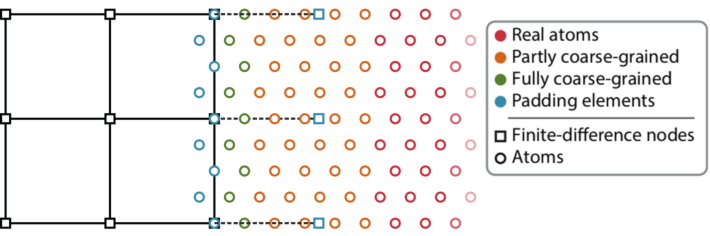
\includegraphics[width=\textwidth]{fig1.pdf}
  \end{center}
  \caption{Schematic representation of the atomistic-continuum interface. The fully atomistic region is represented by real atoms while the fully micromagnetic region is represented by finite-difference nodes. In the interface, both regions mix each other.}
  \label{fig:scheme}
\end{figure}

The solution at padding atoms is obtained by bilinear interpolation of the continuum solution with normalisation. The normalisation is introduced to preserve the length of spin magnetic moments.
The solution at padding nodes is obtained by normalised weighted average of the atomistic solution inside the box with side $\Delta x$ centred at the padding node, where $\Delta x$ is the inter-node distance. For all atoms inside the box, the weight is assigned as the area of the intersection of the box with side $a$ centred at the atom and the box with side $\Delta x$ centred at the padding node. The normalisation is introduced to preserve the nodal length of the vector field solution.

To reduce the ghost-torque error for systems with non-nearest-neighbour atomistic interactions, the behaviour of atoms close to the atomistic-continuum interface is modified \cite{paper2}. More specifically, $J_{ij}$ and ${\bf D}_{ij}$ are modified for a finite set of atoms. Two types of modified atoms can be distinguished --- the fully coarse-grained atoms, which interact only with the nearest neighbours, and the partly coarse-grained atoms, which also interact with non-nearest neighbours. The modification of $J_{ij}$ and ${\bf D}_{ij}$ is performed such that the fully coarse-grained atoms completely isolate the atomistic-continuum interface. More details about the exact way of modifying the atoms can be found in Ref.~\cite{paper2}. 

To reduce the high-frequency wave-reflection from the atomistic-continuum interface, additional numerical damping is added to atoms close to the atomistic-continuum interface \cite{paper1,paper2,paper3}. This damping acts as a low-pass filter for the waves travelling from the atomistic region to the continuum, as the solution is ``attenuated'' to an average solution within a certain window. Due to dispersive nature of the spin waves, the damping is non-linear and depends on time derivative of the solution. The analysis of the dynamics of the damping layer and the exact form of the modification can be found in \cite{paper1}. 

The time stepping was performed simultaneously for all degrees of freedom, i.e. all finite-difference nodes and atoms. The solution at padding atoms/nodes at a certain time step is obtained from the continuum/atomistic solution of the same time step. Mid-point\vindex{Mid-point solver} \cite{dAquino2005} and Depondt\vindex{Depondt solver} \cite{depondt2009spin} methods were used to solve Eqs.~(\ref{eq:ASD_LLG}) and (\ref{eq:C_LLG}) in time.

\section{License}\vindex{License}

The \name{$\mu$ASD} code is developed by the Division of Materials Theory, in the Department of Physics and Astronomy at the University of Uppsala, Sweden. The copyright of the code is help by the developers but the program is open for use and distribution according to the { \b fXXX} license.
 Further information concerning the license and contact information of the developers may be found on the UppASD webpage: \url{http://www.physics.uu.se/UppASD}. The current version of the code (1.0) is still under active development.

\section{Installation}\vindex{Installation}

The source code is distributed along with documentation as part of UppASD and a growing set of examples. To install, perform the following actions.
\begin{gBox}
\begin{enumerate}
\item Obtain the code, by extracting the downloaded archive (or by pulling from the git repository)
\begin{verbatim}
tar xvzf  UppASD_dist.tar.gz
\end{verbatim}
or in the case of git
\begin{verbatim}
git clone github:uppasd
\end{verbatim}
%(\texttt{UppASD_dist.tar.gz}) or alternatively using git (\texttt{git clone github:uppasd}. 
\item Generate the dependencies needed for compiling the code
\begin{verbatim}
make deps
\end{verbatim}
\item (Optional) Perform a system check for available compiler profiles
\begin{verbatim}
make probe
\end{verbatim} 
\item Compile the code with the selected compiler profile
\begin{verbatim}
make <profile>
\end{verbatim}
where \texttt{<profile>}is the name of the profile, i.e. \texttt{ifort}, \texttt{ifort-cuda}, \texttt{gfortran}, \\
\texttt{gfortran-osx}, and so on. Eg. \texttt{make ifort} \\
\item (Optional) Test the compiled program against a selection of realistic runs
\begin{verbatim}
make tests
\end{verbatim}
\end{enumerate}
\end{gBox}

\noindent In addition to the source files, the \name{$\mu$ASD} code as part of UppASD distribution also contains several examples (in the directory \texttt{examples/multiscale}), documentation, including this file (in  \texttt{docs/}) and routines and reference data (\texttt{tests/}) for validating the installation of the \name{$\mu$ASD} code as part of the UppASD program.

\section{Principles of the Code}\vindex{Principles of the Code}

When run, \name{$\mu$ASD} essentially goes through three stages as in UppASD:

\begin{enumerate}
\item Initialization: the system is set up.
\item Initial phase: an optional stage in which the system is brought into thermal equilibrium, with limited data sampling.
\item Measurement phase: the system is evolved in time, with complete data sampling being made.
\end{enumerate}

During the initialization phase, all the parameters necessary to describe the system of interest, such as its geometry, dimensions, exchange couplings and boundary conditions, are set up. In addition, the initial phase also sets the simulation parameters, such as the number of simulation steps to record data over, which SDE solver to use, and the temperature at which the simulation should be run.

The initial phase, which is optional, is typically performed in order to bring the system into thermal equilibrium, so that the data recorded in the measurement phase is for a thermalized system. Obviously, if one is interested in out-of-equilibrium dynamics, then there is no need to perform this phase. In the current version of the code, the initial phase can only be performed using Spin Dynamics (SD).

During the measurement phase, the data sampling is performed. Simulations can be run only in SD mode.

%%%%%%%%%%%%%%%%
\chapter{Input files}\vindex{Input files}
\name{$\mu$ASD} accepts some parameters from command line, but the entire setup is specified in a single file, called \rfilename{multiscale.conf} (if not specified otherwise), that should be placed in the working directory. The output is written in a separate folder called \rfilename{output}. As FORTRAN provides no standard way of creating a directory, the user is responsible of creating it. 

\section {Configuration file}\vindex{Configuration file}
The configuration is contained in a simple text file. There are two kind of parameters; most of them are variables, specified by a name followed by a value (the value may consist of various words, for example, when the variable is a vector or a list). 

The other kind of parameter is the list. Every line after the list header that matches the format of its entries defines an element of the list.
Lists accept the optional \keyword{filename} tag at the end of their header, that must always be followed by file name.
If this tag is present, entries of the list are read from the specified file instead of the main configuration file.
This is recommended for large lists, as it makes reading the configuration easier.

Text after the symbol \verb|#| is ignored, allowing to create comments or, if desired, UNIX shebang headers, to make a configuration file executable.

This is the list of parameters accepted by the configuration file:
\begin{description}[leftmargin=!,labelwidth=\widthof{\bfseries 9999}]
%
\litem{atomistic_shape} {\bf [file <filename>]}  \\Mandatory, list. The shapes that define the atomistic region.This field can be followed by one or many shape specifiers, see \autoref{sec:shapespec}.
 % 
\litem{format} {\bf(P | B | M)}   \label{kw:format} \\Optional, default is set to P. If P, \rfilename{*.dat} files are saved as plain text files. B specifies \rfilename{*.dat} binary files and M represents MATLAB-compatible \rfilename{*.m} files. Plaintext and binary files are valid UppASD input files. Plaintext is easier to work with but generates large files. Binary files are compact and faster to read but hard to modify. MATLAB format is not valid as UppASD input, but is useful for debugging and visualisation purposes. 
%  
\litem{coarse_grained_width} {\bf <nonnegative real>}  \\ Mandatory. Specifies the width of the fully coarse-grained region, the width is measured from the padding atoms. All the atoms closer than the parameter to a padding atom are considered as coarse-grained.
%  
\litem{damping_band_width} {\bf <positive real>}   \\Mandatory. Specifies the width of the damping band. The width is measured from the padding atoms. If 0 is specified, no damping band will be constructed.
 % 
\litem{damping_band_window_size} {\bf<width> <height> <depth>}  \\ Mandatory. Specifies the averaging window size for the damping band. The value of this parameter should depend of the dimensionality, the lattice and the interaction distance. There is a lower bound for this window size, as if there are less than 3,6 or 10 atoms for dimensionality 1,2 and 3 respectively, the calculation of the damping coefficients would involve inverting a singular matrix. MUASD generates NaN's in the damping band coefficients file in this case.
%  
\litem{dimension} {\bf(1 | 2 | 3)}   \\Mandatory. Specifies the dimensionality of the simulation.
 % 
\litem{exchange_atoms} {\bf {[unitcell] [file <filename>]}} \\  Mandatory, list. The exchange between the atoms. See exchange specifiers \autoref{sec:exchangespec}.
%  
\litem{exchange_coarse} {\bf{[unitcell] [file <filename>]}}  \\Mandatory, list. The exchange between the fully coarse-grained atoms. See exchange specifiers \autoref{sec:exchangespec}.
 % 
\litem{finitediff_boxes} {\bf<x> <y> <z>}  \\Mandatory. The number of finite-difference boxes in the direction of each dimension. A box in three dimensions is a cube that have eight finite-difference grid points as its corners. This parameter is used together with the universe size to define $\Delta x$.
 % 
\litem{continuous_exchange_coef} {\bf <real>}   \\Mandatory. Exchange parameter for finite-difference region.
 % 
\litem{continuous_moment_magnitude} {\bf <real>} \\ Mandatory. The magnitude of the moments in the continuous region. The moments of these nodes are initialised to $(\text{magnitude}, 0, 0)$. In order to set up different initial moments, the user can to modify \rfilename{output/moments.dat}.
 % 
\litem{hole_shape} {\bf{[file <filename>]}}  \\ Optional, list. Defines holes in the atomistic region. This field can be followed by one or many shape specifiers, see \autoref{sec:shapespec}.
 % 
\litem{atom_lattice_spacing} {\bf<positive real>}  \\  Mandatory. This parameter is used to approximate the side of the Wigner-Seitz cell around each atom. Each atom is enclosed by a cube of side the value of this parameter. The approximation is used to calculate weights for averaging padding atoms and interface nodes and in the coefficients used in the damping band. The optimal value depends on the lattice.
 % 
\litem{padding_width} {\bf <positive real>} \\ Mandatory. Specifies the width of the padding region, the width is measured from the boundary. Padding atoms serve as reference while placing fully coarse-grained and partially coarse-grained atoms, as well as damping atoms. See \autoref{sec:details:linking} for more details. The value of this parameter should be the interaction radius of fully coarse-grained atoms, plus a small value to prevent numerical issues. This value ensures that all fully coarse-grained atoms have a padding atom for all possible interaction they could have.
 % 
\litem{part_coarse_grained_width} {\bf<nonnegative real>}  \\Mandatory. Specifies the width of the partially coarse-grained region. Those atoms that are closer to a padding atom than the distance \keyword{coarse_grained_width} + \keyword{part_coarse_grained_width} is considered to be partially coarse-grained.
 % 
\litem{periodic_boundary} {\bf(T | F) (T | F) (T | F)} \\  Mandatory. Specifies if the boundary is periodic or not, T indicates a periodic boundary, F indicates an open boundary.
 % 
\litem{universe_size} {\bf<width> <height> <depth>} \\ Mandatory. Specifies the size of the space that the simulation takes place in.
 % 
\litem{unitcell_atoms} {\bf<width> <height> <depth> {[file <filename>]}}  \\Mandatory, list. The width, height and depth are the size of the unit cell. Then a list of the atoms should follow. See Unit cell atoms in \autoref{sec:ucell}.
  %
  \litem{anisotropy} {\bf<anisotropy parameters> {[<anisotropy parameters>]}} \\Optional, list, repeatable. Specifies regions affected by an anisotropy. This line must be followed by shape specifiers (\autoref{sec:shapespec}). The \keyword{anisotropy parameters} are defined as: \\\keywordl{(uniaxial|cubic|both <ratio>) K1 K2 ex ey ez}\\
   The first parameter is the anisotropy type. \keyword{K1} and \keyword{K2} are two real coefficients and \keyword{ex ey ez} is the direction vector $\vec{e}$. It must be specified twice if the flag \keyword{mult_axis} is present in \rfilename{inpsd.dat}. This parameters correspond to what appears in \name{UppASD}'s manual, please refer to it for more details.\cite{uppasddoc} This option is offered as a convenient manner to specify anisotropies, but inputed values are kept unchanged in the output file. If two regions of different anisotropies overlap, the one specified first will take precedence.
\end{description}

\subsection {Shape specifiers}
\label{sec:shapespec}
\keyword{hole_shape}, \keyword{atomistic_shape} and \keyword{anisotropy} can be followed by a list of shapes. These are the recognised shapes:
\begin{description}[leftmargin=!,labelwidth=\widthof{\bfseries 9999}]
%
\litem{box} {\bf<x> <y> <z> <width> <height> <depth>} \\
  Specifies a box with the same dimension as the space. The parameters X Y and Z determine where the corner closest to the origin of the coordinate system will be placed. Width Height and Depth determine the extension of the box in the X, Y and Z directions, respectively.
  Even if the dimension is less than 3, the user must specify all 3 coordinates. The box considers all the coordinates when it decides if a point is inside it or not.

\litem{sphere} {\bf <x> <y> <z> <radius>} \\
  Specifies a sphere of the given radius with centre in (X,Y,Z). As with the box, the user must specify all 3 coordinates regardless of the dimension.
\end{description}

\subsection {Exchange specifiers}\vindex{Exchange specifiers}
\label{sec:exchangespec}
The syntax for the exchange list header is the following:
\syntline{exchange\_atoms [unitcell] [file <filename>]}
This header can be followed by one or more inter-atomic exchange specifiers. If the flag \keyword{file} is present, the specifiers will be read from the given file. Each specifier should be in a separate line, following this format:
\syntline{<Atom type 1> <Atom type 2> <x> <y> <z> <exchange>}
The \keyword{Atom type} fields serve to filter which type of atoms each rule affects. The \keyword{exchange} field specifies the exchange value in mRy.
The meaning of \keyword{x},\keyword{y} and \keyword{z} depends on the flag \keyword{unit cell}

If the flag \keyword{unitcell} is not present in the header, \keyword{x},\keyword{y} and \keyword{z} form a direction vector, representing the relative position between two atoms. For example:\\
\begin{minipage}{\linewidth}
\begin{lstlisting}
  exchange_atoms
  1 1  0.5  0.0 0.0 1.23
  1 1  0.0  0.4 0.0 2.22
  1 1 -0.5  0.0 0.0 1.23
  1 1  0.0 -0.4 0.0 2.22
\end{lstlisting}
\end{minipage}
In this setup, atoms of type 1 are at a distance of 0.5 units each other in the X axis and are aligned with respect to the Y axis will have an exchange parameter of 1.23. Those aligned with respect with the X axis and whose distance is 0.4 will have an exchange parameter of 2.22.

If the \keyword{unitcell} tag is present, the exchange is specified depending on the relative position of the unit cells in which each atom is, instead of the atom position. 
For example:\\
\begin{minipage}{\linewidth}
\begin{lstlisting}
  exchange_atoms unitcell
  1 1   0  0 0 2.22
  1 1   1  0 0 1.23
  1 1  -1  0 0 1.23
  1 1   0  1 0 1.23
  1 1   0 -1 0 1.23
\end{lstlisting}
\end{minipage}
In this setup, atoms that are in the same unit cell receive an exchange parameter of 2.22. Atoms in neighbouring unit cells (using 4-connected neighbourhoods) receive an exchange constant of 1.23. Note that the offsets in this case are integer-valued.


\subsection {Unit cell atoms}\vindex{Unit cell atoms}
\label{sec:ucell}

The syntax for the unit cell header is as follows:
\syntline{unitcell\_atoms <width> <height> <depth> [file <filename>]}
The \keyword{width}, \keyword{height} and \keyword{depth} values refer to the size of the unit cell.
Following this header the user can describe how atoms in the unit cell are.

Each atom is defined by one line in this format:
\syntline{<Atom type> <x> <y> <z> [/] <moment magnitude> <mx> <my> <mz>}
\keyword{Atom type} indicates the type of the atom, used in the exchange specification (see \autoref{sec:exchangespec}).
\keyword{x}, \keyword{y} and \keyword{z} are the coordinates of the atom inside the unit cell. These coordinates are in the interval  [0,1]. The user should avoid placing atoms close to the corners of the cell. This is because otherwise atoms could be placed at the atomistic-continuum boundary, which should not happen. \name{$\mu$ASD} will automatically ignore atoms close to the edges, but it may generate unexpected results if the user is not aware of this. 
Optionally, the user may type a slash(\verb|/|) after the coordinates. This helps with readability of the line.
The value of \keyword{moment magnitude} is length of the magnetic moment vector.
Parameters \keyword{mx}, \keyword{my} and \keyword{mz} are components of a vector parallel to the moment of the atom. There is a constrain in the norm of the vector specified by the user, it can never be shorter than $10^{-3}$ to prevent numerical issues.

In order to calculate the magnetic moment of the atom, the vector (\keyword{mx}, \keyword{my}, \keyword{mz}) is normalised and multiplied by \keyword{moment magnitude}. 

The whole generation process is discussed in \autoref{sec:details:gen}.

\section {Command line}\vindex{Command line}
In the command line, the typical help (\keyword{-{}-help} or \keyword{-h}) and version (\keyword{-{}-version} or \keyword{-v}) options are available. Furthermore, it is possible to get a brief explanation of the input file fields using the help option followed by one or several parameter names.
For example:
%\begin{fBox} 
%\begin{Verbatim}
\begin{lstlisting}
$ ./muasd -h dimension universe_size
option dimension
   Syntax: dimension (1 | 2 | 3)
   Specifies the dimensionality of the simulation.
option universe_size
   Syntax: universe_size <x> <y> <z>
   Specifies the size of the space that the simulation takes place in.
   \end{lstlisting}
%\end{Verbatim}
%\end{fBox} 

It is also possible to select an alternative configuration file (other than \rfilename{multiscale.conf}). This is done by passing the name of the configuration file as an argument.

\section{CheckPositions}\vindex{checkPositions}
\name{CheckPositions} is a MATLAB program bundled with \name{$\mu$ASD}. After running \name{$\mu$ASD} you can change your working directory to \rfilename{./output} in  MATLAB and run there \name{checkPositions}. In order to run \name{checkPositions} from any directory, use the command \verb|addpath('path/to/checkpositions');|.

To run \name{checkPositions} it is required that the format of the output is set to MATLAB (\keyword{format m}, See \autoref{kw:format}).

In 1D, \name{checkPositions} adds an offset in the \rfilename{Y} coordinate of the plot for different kinds of elements. This eases reading atom indices and prevents atoms from occluding each other. See an example in \autoref{fig:1d_example}
\begin{figure}[!h]
	\centering
	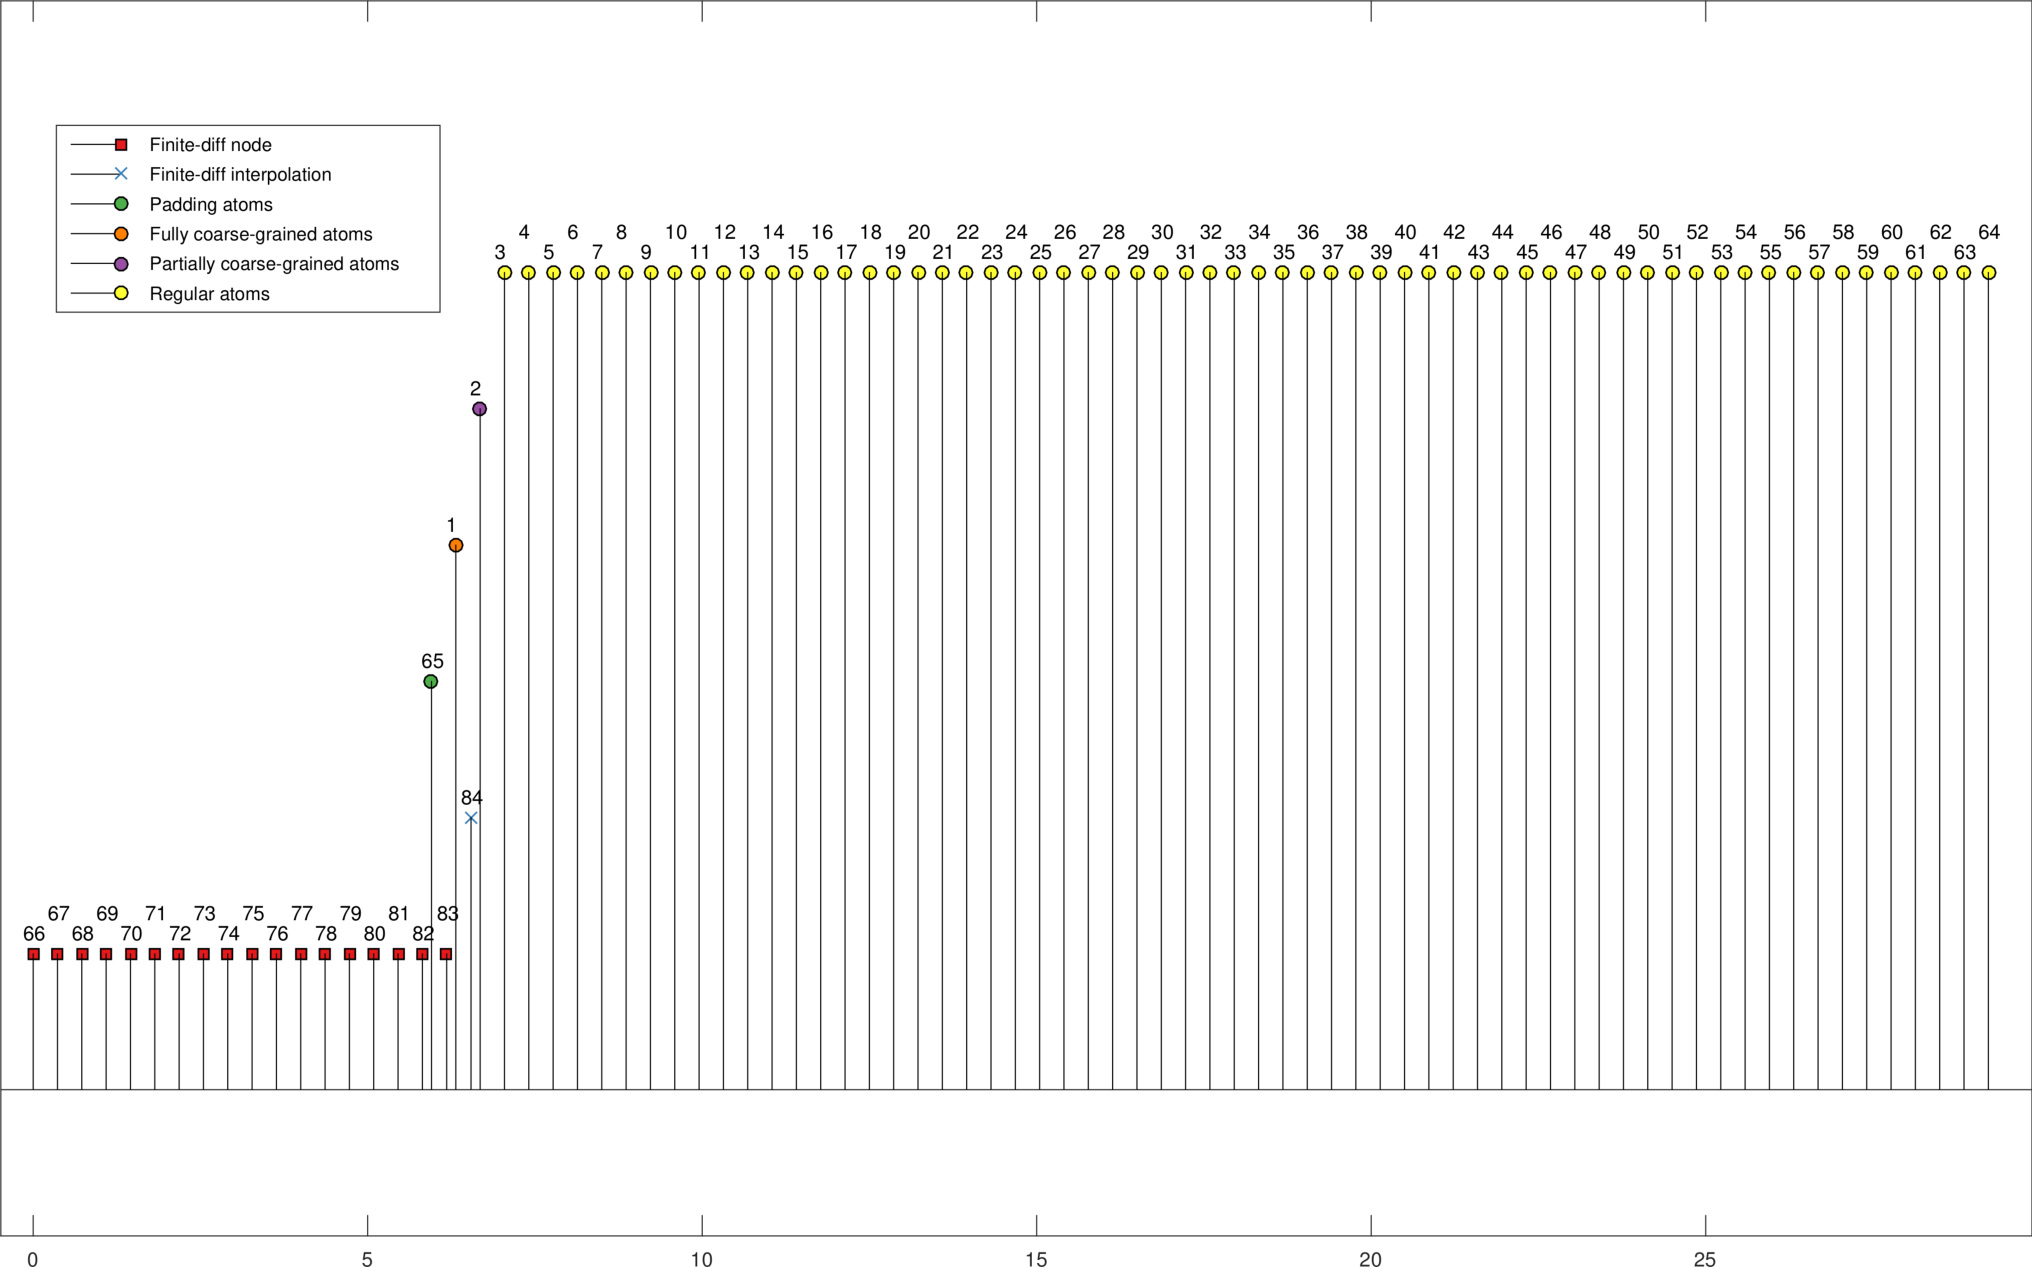
\includegraphics[width=\textwidth]{example1d.pdf}
	\caption{1D Example, checkPositions plot.}
	\label{fig:1d_example}
\end{figure}


\chapter{Basic examples}\vindex{Basic examples}
Some typical examples of simulations using the \name{$\mu$ASD} software is discussed here in rather great detail. 

\section {1D strip}\vindex{1D strip}
This example shows how to set up a 1D strip with an atomistic and a continuum region.

\lstinputlisting[mathescape]{examples/multiscale-1d}

\noindent The first line specifies the dimensionality, this is a 1D simulation.\\
Lines 2,3,4 and 5 let the user specify the thickness of each atomistic layer.\\
Line 6 specifies that periodic boundary conditions are not used for either direction. \\
Line 7 sets the size of the universe. Only the first coordinate is considered, as the example is 1-dimensional. \\
Line 8 defines the number of boxes in which the universe will be split. \name{$\mu$ASD} first covers the whole space with finite difference boxes, then turn some of those boxes inside atomistic boxes. Later finite difference nodes are placed in the corners of finite difference boxes and the unit cell is tiled inside atomistic boxes. The finite difference lattice spacing is the element-wise division between \keyword{universe_size} and \keyword{finitediff_boxes}, in this case $0.3636$.\\
Line 9 sets the atomistic lattice spacing. As the unit cell contains only one atom, the interaction distance will also be 0.3636 (specified in line 10). For more details on how this parameter is used see \autoref{sec:detail:dband}.\\
Line 10 specifies the exchange parameter for the finite-difference region. Note that this is a parameter in the PDE, i.e. nodes interact with the value scaled by $\Delta x^2$.\\
Line 11 establishes the magnetic moment magnitude in the finite-difference region. Remember that all magnetic moments are pointing towards $+x$ unless \rfilename{moments.dat} is modified.\\
Line 12 defines an averaging window size for calculating the damping band coefficients.\\
Line 14 will cause the output to be compatible with GNU Octave/MATLAB. This is required for plotting the setup \name{checkPositions}.\\
Line 16 starts the \keyword{unitcell_atoms} list. Its parameter is the dimension of the cell, in this case $0.3636$, same as the finite-difference lattice spacing. The next line adds one atom to the unit cell, of type $1$, located at $x=0.5$ and magnetic moment magnitude $5$ towards $+x$.\\
Line 19 contains the header of the \keyword{atomistic_shape} list. In line 20 we have the single element that this list holds, in this case a sphere centred in $(29.4516,0,0)$ and of radius $23.2741$. The centre corresponds to the universe size, so it will be in one end of the space. The radius spans $23.27/0.3636$, a bit more than $63$ unit cells.\\
Line 22 defines the interactions between atoms. We are using position offsets instead of unit cell offsets in this case. Lines 23 and 24 specify interaction rules from an atom \emph{A} to an atom \emph{B}. Note that the interactions are not symmetric. The first two numbers select the type of atoms \emph{A} and \emph{B} respectively. The next three numbers filter atoms by their relative positions. Let's call these numbers $d_x$,$d_y$ and $d_z$, then, only if $B-A \approx (d_x,d_y,d_z)$ the interaction will occur. The last value is the exchange parameter, in mRyd.\\
Lines 26, 27 and 28 work in the same way. These lines represent the exchange used for fully coarse-grained atoms.

\section{2D example}\vindex{2D example}\label{2d}
This example shows how to set up a 2D simulation with an atomistic and a continuum region.
\lstinputlisting[mathescape]{examples/multiscale-2d}

See in \autoref{fig:2dperiodicexample}-a) how the setup will be generated. The squares in the figure are finite-difference nodes, the crosses are also finite-difference nodes but there moments will be interpolated from the atoms that surround them. Thus those interpolated nodes work as boundary conditions for the other finite-difference nodes. The yellow points are real atoms, inside the atomistic region. As we approach the continuum we see purple (partially coarse-grained) atoms. There is one layer of them, since \keyword{part_coarse_grained_width} roughly exceeds the atomistic lattice spacing. The next row, in orange, represents fully coarse-grained, again only one layer is generated.
The green layer is already outside the atomistic region and represents padding atoms. Those atoms are interpolated by their closest four finite difference nodes (red squares in the picture). Inside the atomistic region there is one layer of finite difference interpolation nodes. These nodes are interpolated with their surrounding atoms, see more details in \autoref{sec:details:interpolation}.

If boundary condition is used along the vertical direction then the setup becomes as in \autoref{fig:2dperiodicexample}-b). We can see that the continuum nodes disappear at the top of the setup, to avoid duplicate nodes. The continuum nodes that are at the bottom of the setup will be linked to those nodes that are closest to the top boundary in this setup.

The green strip of atoms that appeared at the top-centre of the setup is made of padding atoms, these appeared due to the orange (fully coarse-grained) atoms at the bottom boundary.
\begin{figure}[htp]
\centering
\begin{tabular}{cc}
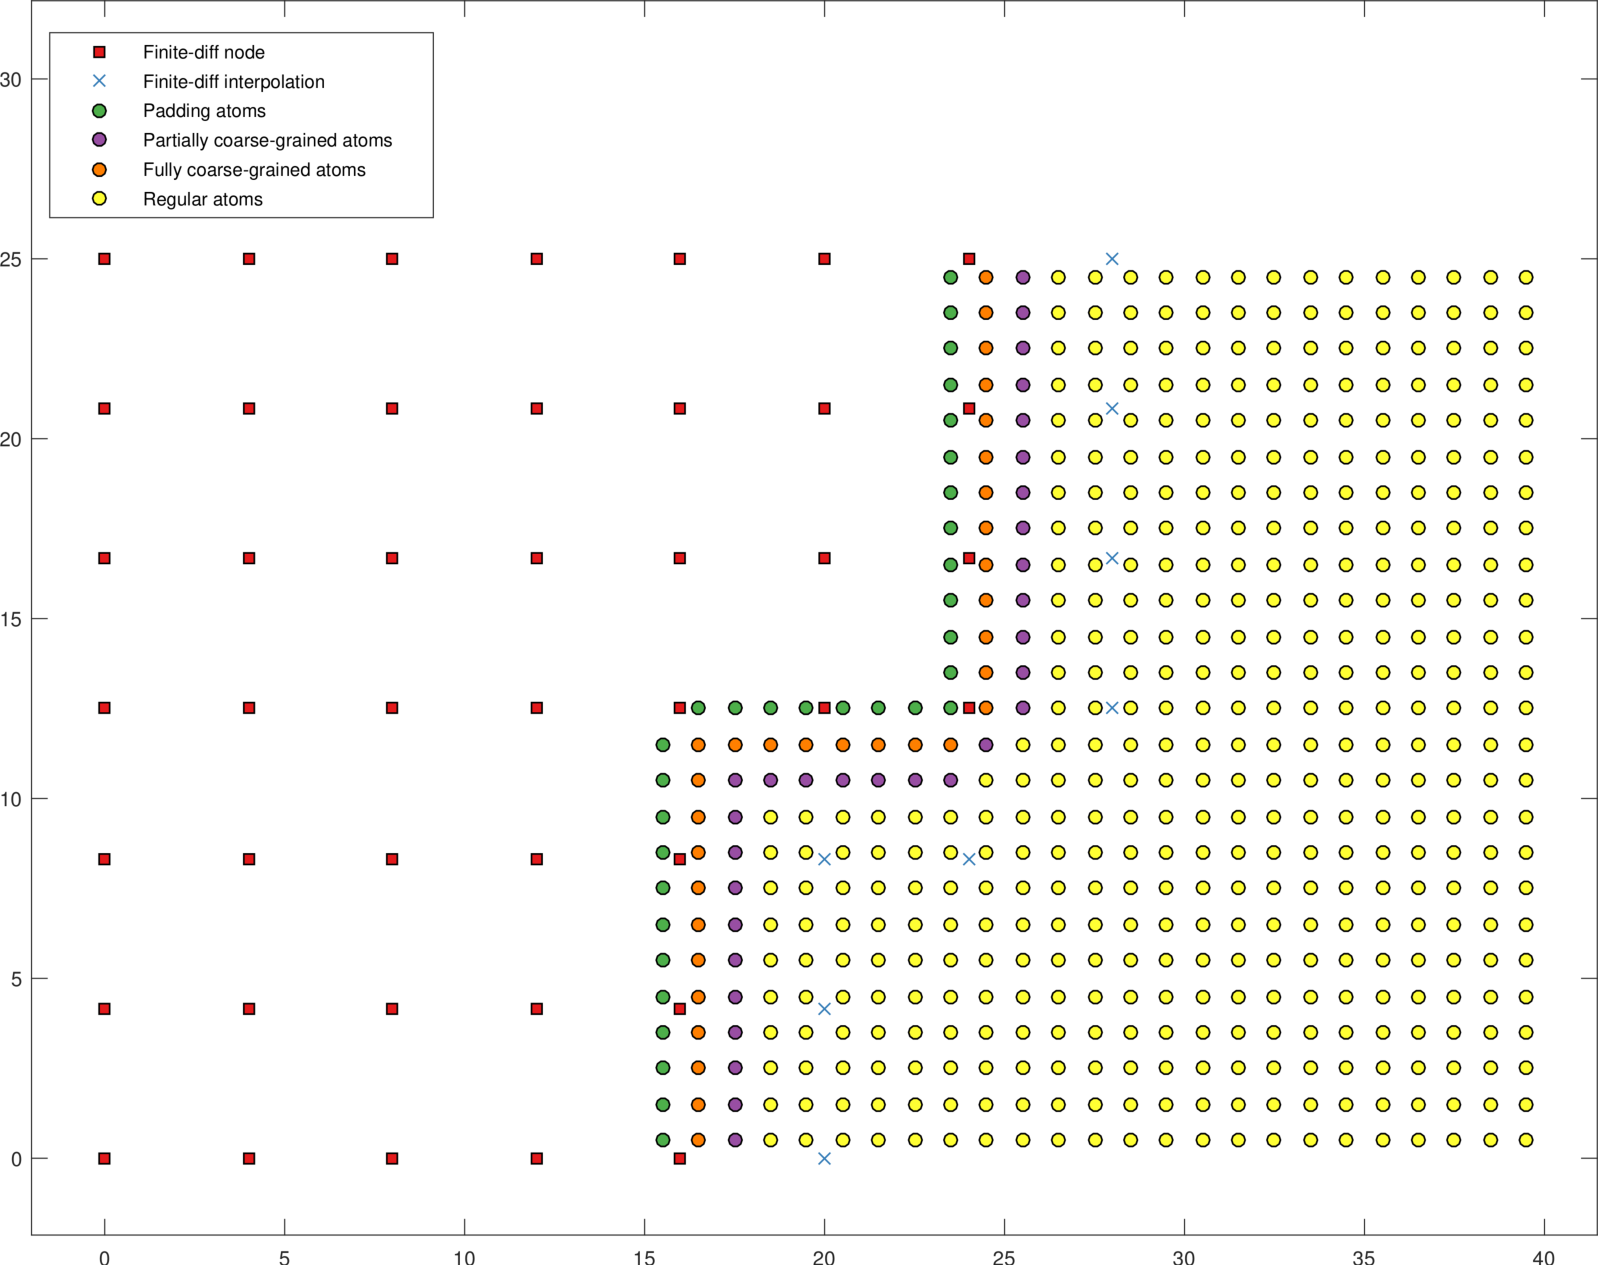
\includegraphics[width=72mm]{2dexample.pdf}&
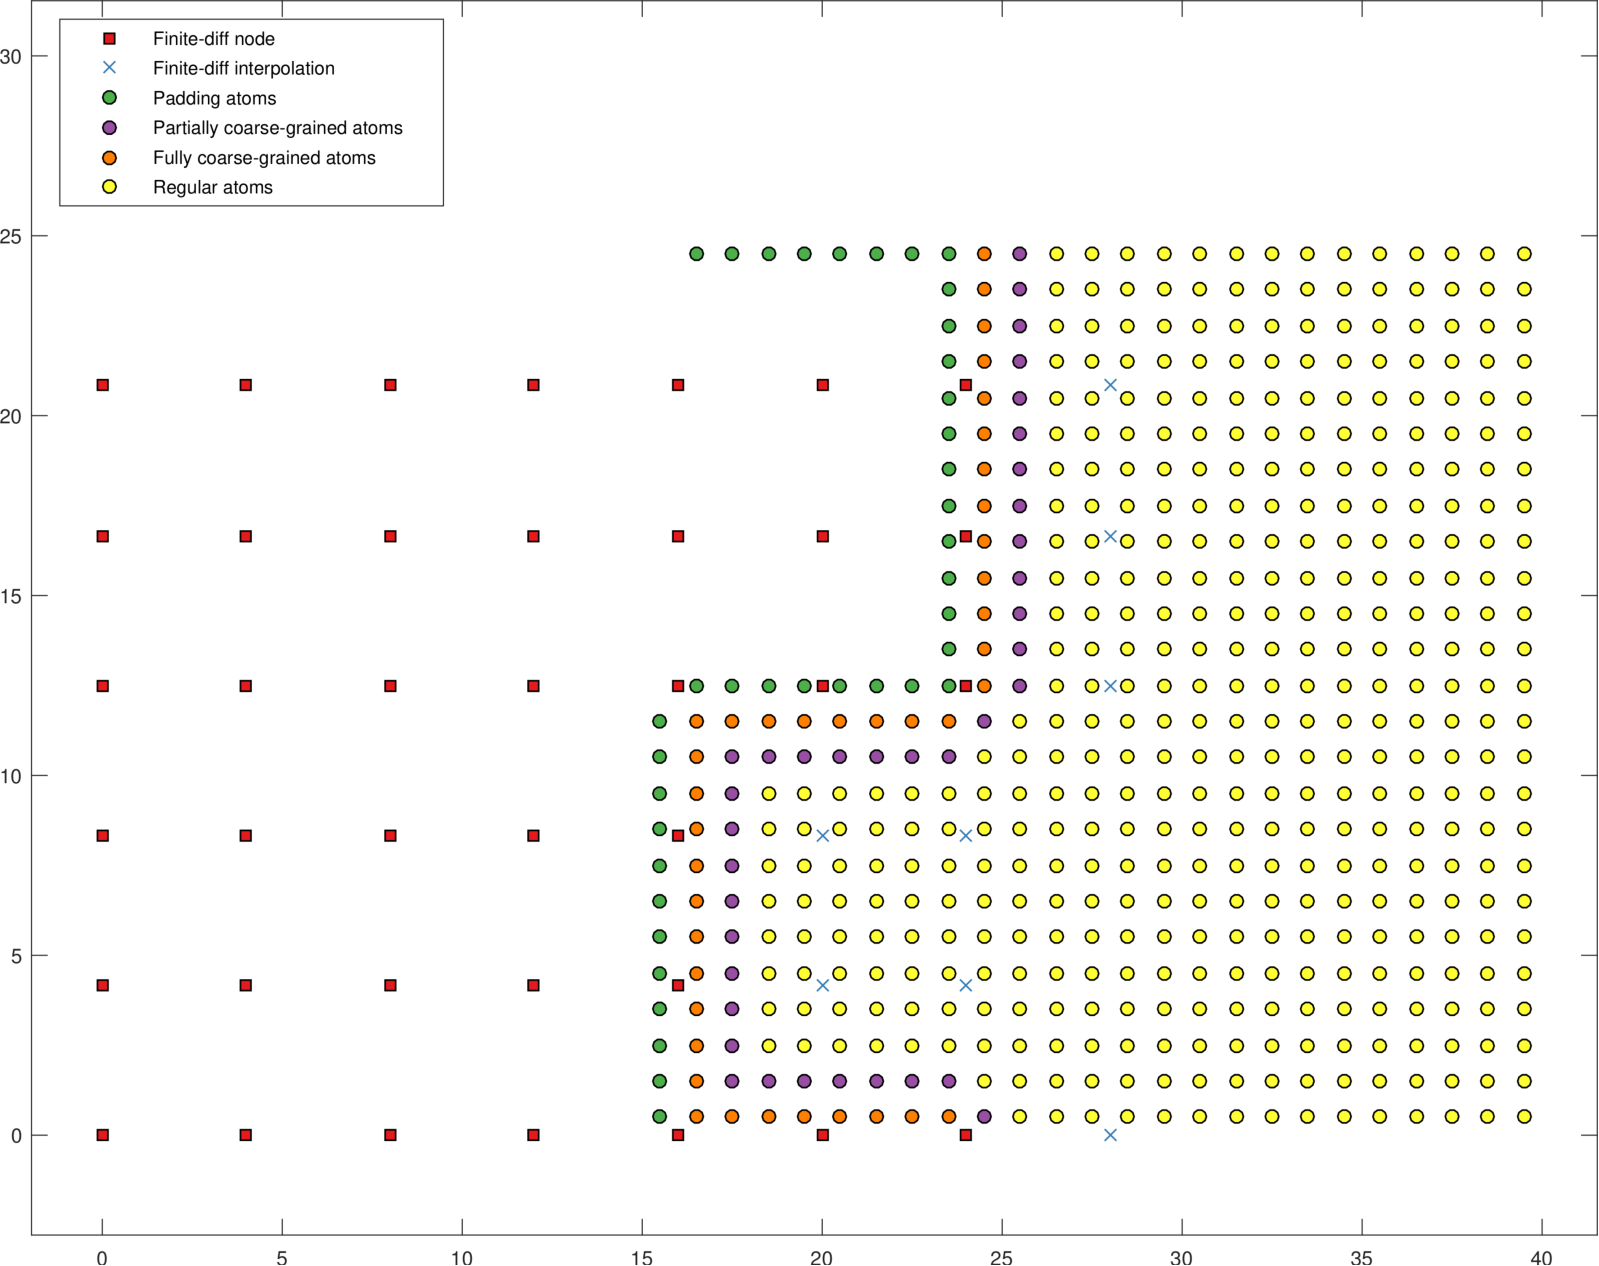
\includegraphics[width=72mm]{2dperiodicexample.pdf}
\end{tabular}
\caption{a) 2D example with open boundary conditions (left panel). b) 2D example with periodic boundary condition in the vertical direction (right panel).}
\label{fig:2dperiodicexample}
\end{figure}


\section{3D example}\vindex{3D example}
This example shows a 3D simulation with an atomistic spherical region in the centre, surrounded by the continuum region. In Fig.~\ref{fig:example3d} is shown a 3D distribution of the atoms in the interval $[25,50]$ along the x, y and z cartesian coordinates.
\lstinputlisting[mathescape]{examples/multiscale-3d}

This example also includes a hole in the middle of the space. The hole is specified in lines 15 and 16 as a sphere of centre $\left(25,25,25\right)$ and radius 5.0. Also notice that the interaction rules for the Z axis have been added for both coarse-grained atoms (from line 32) and regular atoms (from line 24). The rest of the setup is very similar to the previous one in \autoref{2d}. 

\begin{figure}[h!]
	\centering
	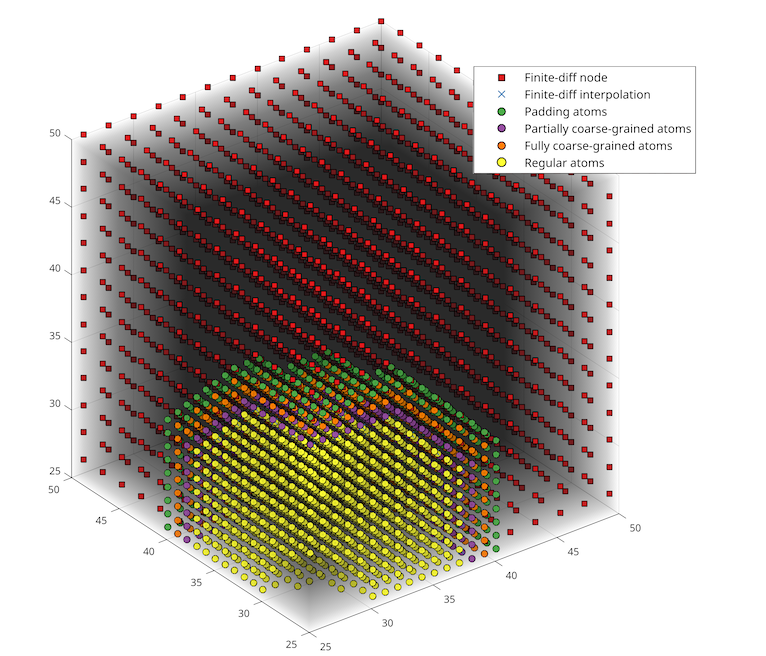
\includegraphics[width=\textwidth]{example3d.png}
	\caption{3D example. For better visualisation only atoms in the interval $[25,50]$ are plotted.}        
	\label{fig:example3d}
\end{figure}


\chapter{Implementation details}\vindex{Implementation details}

\section {System generation}\vindex{System generation}
\label{sec:details:gen}
At first, the finite-difference mesh  is created. The boxes within the mesh are marked as either atomistic or continuum. A box is marked as continuum if one of its corners is inside an atomistic shape.
Thereafter the atoms are generated from the unit cell. The unit cell is repeated over the entire universe and atoms that are inside atomistic boxes are kept, while other atoms are disregarded. Note that there is a small region between atomistic and the continuum domains where atoms are always discarded. This is done to avoid placing atoms exactly on the boundary between the atomistic region and the continuum region. This should not be allowed because, as continuum nodes are always placed in the boundary, atoms overlapping with nodes may appear. This would generate a region that is described by both models, which may not perfectly agree in the result.

The next step is generating padding atoms. These atoms work as boundary conditions for the atomistic part. They are generated exactly as the real atoms, however they are added to the system if they are in the continuum region and if the distance to the closest regular atom is small enough. This distance can be specified in the input file using the keyword \keyword{padding_width}.

\subsection*{Related routines}\vindex{Related routines}
%\renewcommand{\keyword}[1]{\texttt{#1}}
\renewcommand*\DTstylecomment{\rmfamily}
\renewcommand*\DTstyle{\ttfamily\keywordl}
\dirtree{%
  .1 multiscale_setup\DTcomment{multiscale_setup.f90}.
  .2 createFiniteDiffMesh\DTcomment{finitedifference.f90}.
  .3 (auxiliar functions)\DTcomment{finitedifference.f90}.
  .2 createAtoms\DTcomment{multiscale_setup.f90}.
  .3 generateAtoms\DTcomment{atomgenerator.f90}.
  .3 generatePaddingAtoms\DTcomment{atomgenerator.f90}.
  .3 extractFromUnitcellLocation\DTcomment{atomgenerator.f90}.  
  .3 generateFiniteDifferenceAtoms\DTcomment{atomgenerator.f90}.
  .3 (auxiliar functions)\DTcomment{atomgenerator.f90}.
}
\section{Atom linking}\vindex{Atom linking}
\label{sec:details:linking}
The non-padding atoms are divided into three separate regions, the coarse-grained atoms, the partially coarse-grained atoms and the real atoms. The coarse-grained atoms are selected from the generated atoms if their distance to a padding atom is less than \keyword{coarse_grained_width}. The partially coarse-grained atoms are selected by choosing those atoms that are closer to a padding atom than \keyword{part_coarse_grained_width} but are not closer than \keyword{coarse_grained_width}. The remaining atoms are the real atoms. For details about these three atom categories see \cite{paper2}.

After the regions have been initialised, the linking takes place. The coarse-grained atoms are linked only to their nearest neighbours using an exchange derived from \keyword{exchange_coarse}. The linkage in real atoms is done as specified by the user with \keyword{exchange_atoms}. Partially coarse-grained atoms receive their exchange coefficients in function of their position and the exchange used in fully coarse-grained and real atoms, thus providing a smooth transition between these two regions\cite{paper2}.

\subsection*{Related routines}\vindex{Related routines}

\renewcommand*\DTstylecomment{\rmfamily}
\renewcommand*\DTstyle{\ttfamily\keywordl}
\dirtree{%
  .1 multiscale\_setup\DTcomment{multiscale_setup.f90}.
  .2 createRegions\DTcomment{multiscale_setup.f90}.
  .2 setupLinks\DTcomment{multiscale_setup.f90}.
  .3 createFiniteDiffLinks\DTcomment{finitedifference.f90}.
  .3 createExchangeMatrix\DTcomment{atomlinker.f90}.
  .4 (auxiliar functions)\DTcomment{atomlinker.f90}.
}
\section {Interpolation}\vindex{Interpolation}
\label{sec:details:interpolation}

There are finite-difference nodes placed inside the atomistic region, these are only used as boundary conditions for the continuum part. These nodes appear as a blue cross in checkPositions (see \autoref{fig:2dperiodicexample}-a)). The magnetic moment for these nodes is obtained by interpolation of the atoms that surround them. The interpolation is just a weighted average of the atomistic values. To calculate the weights for the atoms, a bounding box, of side the finite-difference spacing, is placed around the finite-difference node. The volume of the intersection between the atom's Wigner-Seitz cell and the bounding box is taken as the weight.

The intersection between the bounding box and  the Wigner-Seitz cells is done by an iterative partitioning method: Let B be a box of equal to the bounding box. If not all corners of B have as one of their closest neighbours the same node, the box is split in every dimension, yielding 2 subboxes in 1D, 4 in 2D and 8 in 3D. The process is repeated taking each subbox as B, until all nodes share a nearest-neighbour or a depth limit is reached. The volume of the subboxes is finally divided and accumulated for each closest neighbours of each corner. This approximation is accurate with a small depth limit, but is still the slowest point in \name{$\mu$ASD} for a large enough interpolation. 

The padding atoms are interpolated from the finite difference-nodes that enclose them in a box. That is, the corners of the finite-difference box in which the padding atom is located.

\subsection*{Related routines}\vindex{Related routines}
\renewcommand*\DTstylecomment{\rmfamily}
\renewcommand*\DTstyle{\ttfamily\keywordl}
\dirtree{%
  .1 multiscale\_setup\DTcomment{multiscale_setup.f90}.
  .2 setupInterpolationWeights\DTcomment{multiscale_setup.f90}.
  .3 createFiniteDiffInterpolationLinks\DTcomment{atomlinker.f90}.
  .4 iterativeAreaCoefficients\DTcomment{areacoefficients.f90}.
  .3 createPaddingInterpolationWeights\DTcomment{atomlinker.f90}.
}

\section {Damping band}\vindex{Damping band}
\label{sec:detail:dband}
The damping band is a low-pass filter that damps high frequency perturbations travelling from the atomistic to the continuum region. The damping band can be applied as an additional term in the effective field in the following way:

  \begin{equationB}[Damping band in the LLG equation]\vindex{Damping band in LLG}
  \begin{align*}
    \frac{\partial\vec{m}}{\partial t} &= \beta_L\vec{m}_i\times\vec{H}_i-\alpha_L\vec{m}_i\times\left(\vec{m}_i\times{\vec{H}_i}\right) - \gamma_{Di}\vec{m}_i \times \left(\vec{m}_i\times\vec{m}_{Ai}\right),\\
     p_{ij} &= \left(\frac{r_i^r}{r_i^r + r_j^p - a}\right)^2 ,\\
     \gamma_{Di} &= g_D\cdot p_{ij}\sqrt{\left|\frac{d}{dt}\vec{m}\right|}.
      \end{align*}
  \end{equationB}
  
\noindent For more details refer to the paper of the method\cite{paper2}. The coefficient $g_D$ is a parameter (\keyword{dband}) the user can directly specify in UppASD, in the file \rfilename{inpsd.dat}. The vector $m_{A_i}$ is the normalized result of a weighted sum of neighbouring vectors. The position-dependent term $p_{ij}$ and the coefficients for calculating $m_{A_i}$ are evaluated in \name{$\mu$ASD} and written into the file \rfilename{dampingband.dat}.

\begin{figure}[b!]
	\centering
	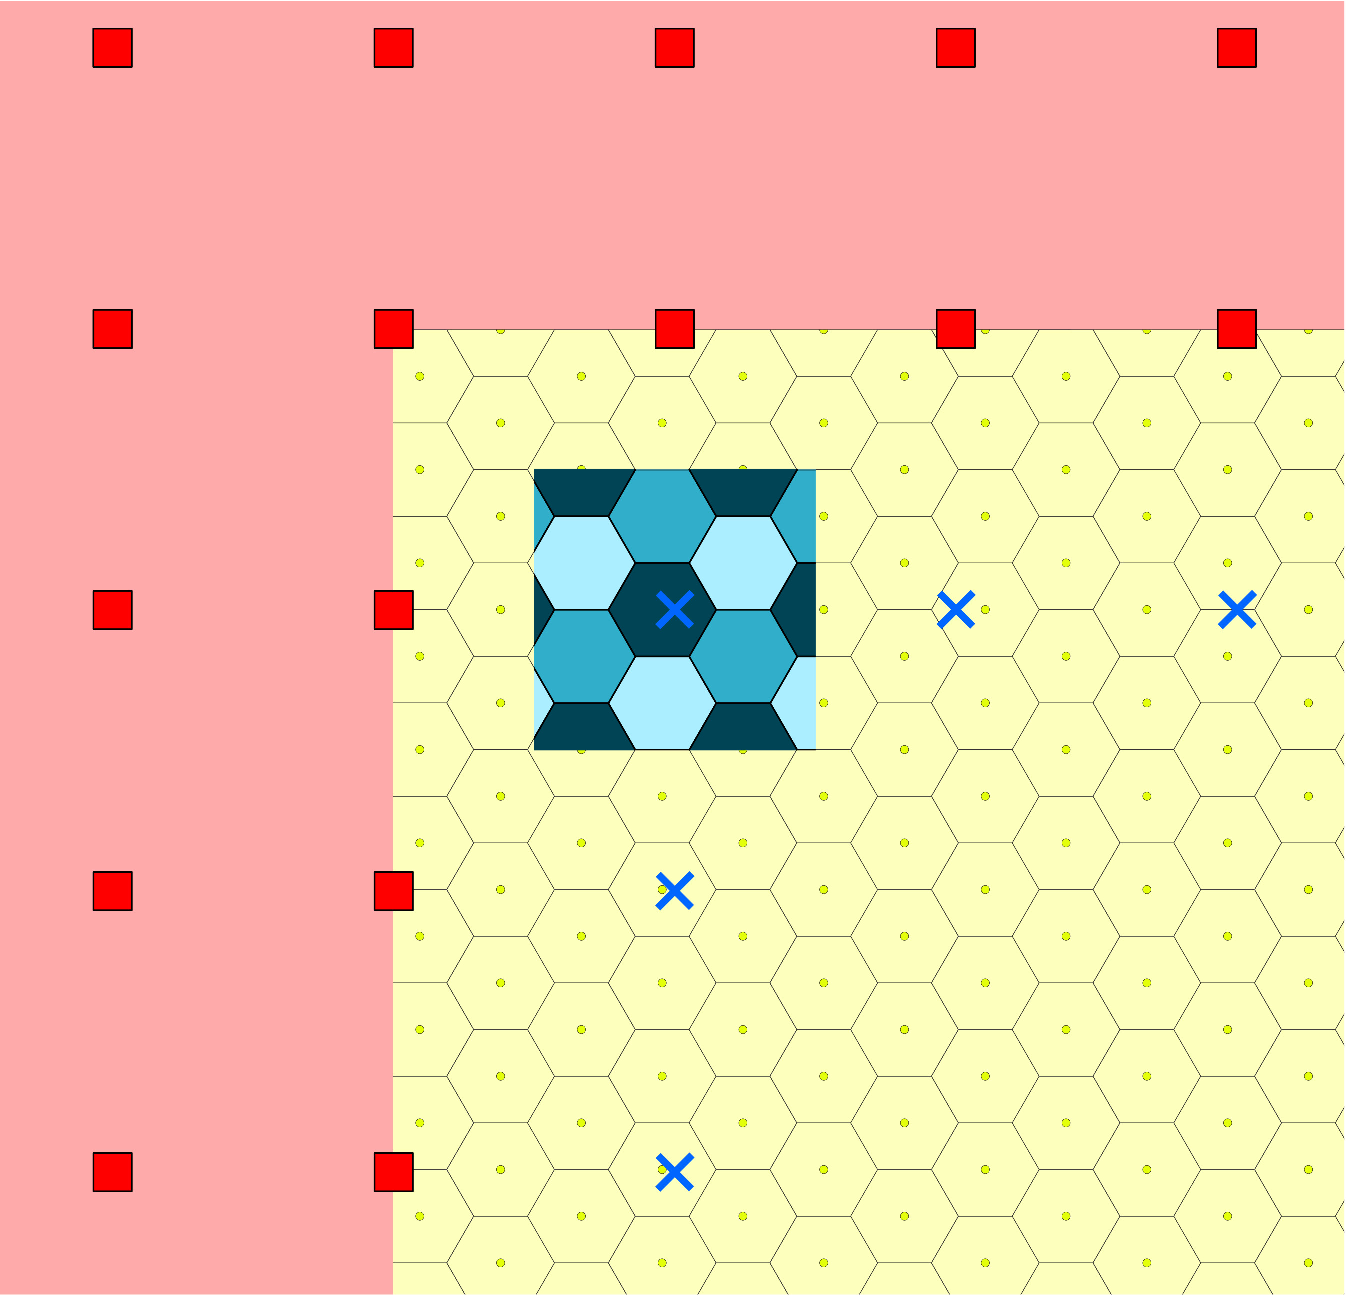
\includegraphics[width=12cm]{interpolationnode.pdf}
	\caption{Two-dimensional bcc lattice. In patterned blue, area that each atom contributes to the interpolation node in the center. In yellow atoms and their Wigner-Seitz (Voronoi) cell.}
	\label{fig:areas}
\end{figure}


In a similar way as the interpolation, damping band coefficients depend on the Wigner-Seitz cell area. In this case finite-difference nodes are also assigned an area, since the interpolation involves magnetic moments from both domains (see Fig.~\ref{fig:areas}). However, the number of atoms affected by the damping band is larger than in the interpolation, and the computation of voronoi areas as described in the interpolation is computationally too expensive. In order to reduce calculation time, \name{$\mu$ASD} approximates the areas, taking a square of side \keyword{atom_lattice_spacing} for each atom instead of its voronoi cell (see Fig.~\ref{fig:boxesareas}). Continuum nodes are circumscribed by boxes of side $\Delta x$. This approximation comes at a cost: not all lattices are ideally represented for the damping band. Cubic lattices are resolved almost perfectly, while some lattices cause holes or intersections between boxes, introducing some error.

\begin{figure}[h!]
	\centering
	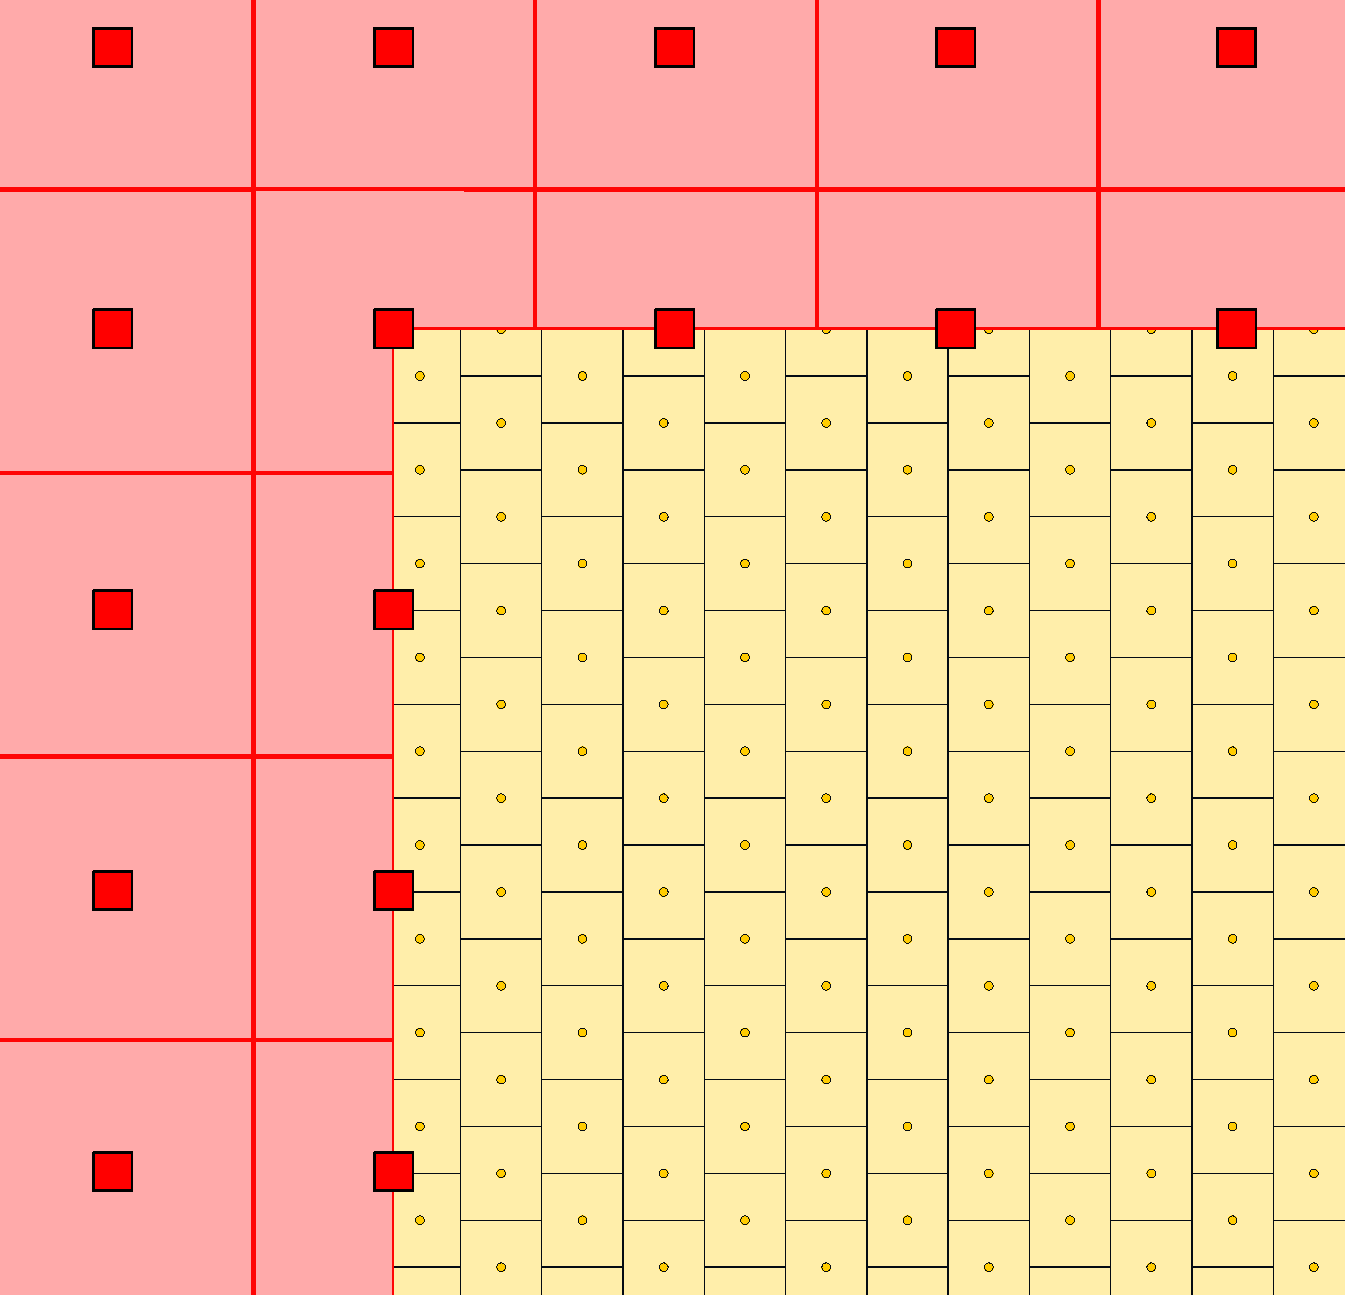
\includegraphics[width=12cm]{dbandinterp.pdf}
	\caption{Boxes approximation in the same setup as \autoref{fig:areas}. In yellow, boxes approximating Wigner-Seitz cells for each atom. In red areas corresponding to each finite-difference node. Note that atomistic and continuum cells never have effect outside their own domain.}
	\label{fig:boxesareas}
\end{figure}

\subsection*{Related routines}
\renewcommand*\DTstylecomment{\rmfamily}
\renewcommand*\DTstyle{\ttfamily\keywordl}
\dirtree{%
  .1 multiscale\_setup\DTcomment{multiscale_setup.f90}.
  .2 setupDampingBand\DTcomment{multiscale_setup.f90}.
  .3 dampingPositionalCoefficients\DTcomment{dampingband.f90}.
  .3 dampingAreaCoeff\DTcomment{dampingband.f90}.
  .4 boxesAreaCoefficients\DTcomment{areacoefficients.f90}.
}


%----------------------------------------------------------------------------------------
%	BIBLIOGRAPHY
%----------------------------------------------------------------------------------------
\begin{thebibliography}{1}

\bibitem{Skubic2008}
B.~Skubic, J.~Hellsvik, L.~Nordstr{\"o}m, and O.~Eriksson\\
%\newblock A method for atomistic spin dynamics simulations: implementations and examples.
\newblock {J. Phys.: Condens. Matter}  \textbf{20}, 315203 (2008).

\bibitem{Antropov1996}
V.~P. Antropov, M.~I. Katsnelson, B.~N. Harmon, M.~van Schilfgaarde, and
  D.~Kusnezov \\
%\newblock Spin dynamics in magnets: Equation of motion and finite temperature effects.
\newblock {Phys. Rev. B} \textbf{54}, 1019 (1996).

\bibitem{Garcia-Palacios1998}
J.~L. Garc\'\i{}a-Palacios and F.~J. L\'azaro\\
%\newblock Anisotropy effects on the nonlinear magnetic susceptibilities of superparamagnetic particles.
\newblock {Phys. Rev. B} \textbf{ 55}, 1006 (1997).

\bibitem{Watson1969}
R.~E. Watson, M.~Blume, and G.~H. Vineyard\\
%\newblock Spin motions in a classical ferromagnet.
\newblock { Phys. Rev.} \textbf{ 181}, 811 (1969).

\bibitem{Eriksson2017}
O.~Eriksson, A.~Bergman, L.~Bergqvist, and J.~Hellsvik\\
\newblock {\it Atomistic {S}pin {D}ynamics - {F}oundations and {A}pplications}.\\
\newblock Oxford University Press, Oxford, 1st edition (2017).

\bibitem{paper1}
  M. Poluektov, O. Eriksson, and G. Kreiss\\
   \newblock{Commun. Comput. Phys.} \textbf{20}, 969 (2016).
   
\bibitem{paper2}
  M. Poluektov, O. Eriksson, and G. Kreiss\\
  \newblock{Comput. Methods Appl. Mech. Engrg.} \textbf{329}, 219 (2018).
  
  \bibitem{paper3}
   \'E. M\'endez, M. Poluektov, G. Kreiss, O. Eriksson, and M. Pereiro\\
   \newblock{Phys. Rev. Research} \textbf{2}, 013092 (2020).
   
   \bibitem{uppasddoc}
  See {\it Uppsala Atomistic Spin Dynamics User Guide.}

   
 \bibitem{Luskin2013}
  M. Luskin and C. Ortner\\
   \newblock{Acta Numerica} \textbf{22}, 397 (2013).
  
  \bibitem{dAquino2005}
  M. d'Aquino, C. Serpico, and G. Miano\\
   \newblock{J. Comp. Phys.} \textbf{209}, 730 (2005). 
   
   \bibitem{depondt2009spin}
  Ph. Depondt and F. G. Mertens\\
   \newblock{J. Phys.: Condens. Matter} \textbf{21}, 336005 (2009). 

\end{thebibliography}

%----------------------------------------------------------------------------------------
%	INDEX
%----------------------------------------------------------------------------------------

\cleardoublepage
\phantomsection
\setlength{\columnsep}{0.75cm}
\addcontentsline{toc}{chapter}{\textcolor{ocre}{Index}}
\printindex

%----------------------------------------------------------------------------------------

\end{document}
